\section{Vị trí tương đối giữa hai mặt phẳng}

\subsection{Đề số 1}
\Opensolutionfile{ans}[ans/ans-1-C4-B4-De1]
\caulc
\begin{ex}%[1H4N4-1]
Tìm khẳng định {\bfseries sai} trong các khẳng định sau đây?
\choice
{Nếu hai mặt phẳng song song cùng cắt mặt phẳng thứ ba thì hai giao tuyến tạo thành song song với nhau}
{Ba mặt phẳng đôi một song song chắn trên hai đường thẳng chéo nhau những đoạn thẳng tương ứng tỉ lệ}
{Nếu mặt phẳng $(P)$ song song với mặt phẳng $(Q)$ thì mọi đường thẳng nằm trên mặt phẳng $(P)$ đều song song với mặt phẳng $(Q)$}
{\True Nếu mặt phẳng $(P)$ có chứa hai đường thẳng phân biệt và hai đường thẳng đó cùng song song song với mặt phẳng $(Q)$ thì mặt phẳng $(P)$ song song với mặt phẳng $(Q)$}
\loigiai{
``Nếu mặt phẳng $(P)$ có chứa hai đường thẳng phân biệt và hai đường thẳng đó cùng song song song với mặt phẳng $(Q)$ thì mặt phẳng $(P)$ song song với mặt phẳng $(Q)$'' là mệnh đề sai khi hai đường thẳng đó song song với nhau.}
\end{ex}

\begin{ex}%[1H4N4-2]
Cho hình chóp $S.ABCD$ có đáy $ABCD$ là hình bình hành. Gọi $M$, $N$, $K$ lần lượt là trung điểm các cạnh $AB$, $BC$, $SB$. Chọn khẳng định đúng trong các khẳng định dưới đây.
\choice
{\True $\left(MNK\right)\parallel \left(SAC\right)$}
{$\left(MNK\right)\parallel \left(SAD\right)$}
{$\left(MNK\right)\parallel \left(SCD\right)$}
{$\left(MNK\right)\parallel \left(SAB\right)$}
\loigiai{
\immini{Ta có $MK$ là đường trung bình của tam giác $SAB$ nên $MK\parallel SA$. \hfill $(1)$\\
Ta có $NK$ là đường trung bình của tam giác $SBC$ nên $NK\parallel SC$. \hfill $(1)$\\
Từ $(1)$ và $(2)$ suy ra $\left(MNK\right)\parallel \left(SAC\right)$.}{\begin{tikzpicture}[scale=1, font=\footnotesize, line join=round, line cap=round,>=stealth]
\path (0,0)coordinate (D)++(3.5,0) coordinate (C)++(1.5,1) coordinate (B) ($(B)+(D)-(C)$) coordinate (A) (0.7,2.5) coordinate (h) ($(A)+(h)$) coordinate (S) (barycentric cs:A=1,B=1) coordinate (M) (barycentric cs:C=1,B=1) coordinate (N) (barycentric cs:S=1,B=1) coordinate (K);
\draw (S)--(D)--(C)--(B)--cycle (S)--(C) (N)--(K);
\draw[dashed] (S)--(A)--(D) (C)--(A)--(B) (K)--(M)--(N);
\foreach \p/\g in {A/150,D/240,C/-60, B/0, S/90,M/30,N/-30,K/30} \fill[black] (\p) circle(1pt)+(\g:0.3) node{$\p$};
\end{tikzpicture}}
}
\end{ex}

\begin{ex}%[1H4N5-1]
Cho hình hộp $ABCD.A'B'C'D'$. Trong các khẳng định sau, khẳng định nào \textbf{sai}?
\choice
{$\left(ABCD\right)\parallel \left(A'B'C'D'\right)$}
{$\left(AA'D'\right)\parallel \left(BCC'\right)$}
{\True $\left(BDD'\right)\parallel \left(ACC'\right)$}
{$\left(ABB'\right)\parallel \left(CDC'\right)$}
\loigiai{
\immini{Gọi $O$ là giao điểm của $AC$ và $BD$. \\
Khi đó, $O\in (BDD')\cap (ACC')$ nên $(BDD')$ không song song với $(ACC')$. }{\begin{tikzpicture}[scale=1, font=\footnotesize, line join=round, line cap=round,>=stealth]
\path (-0.5,2) coordinate (h) (0,0)coordinate (B)++(2.5,0) coordinate (C)++(1,0.8) coordinate (D) ($(B)+(D)-(C)$) coordinate (A) (barycentric cs:A=1,C=1) coordinate (O);
\foreach \p in {A,B,C,D}\path ($(\p)+(h)$) coordinate (\p');
\draw (A')--(B')--(B)--(C)--(D)--(D')--cycle (B')--(C')--(D') (C)--(C');
\draw[dashed] (B)--(A)--(D)--(B) (C)--(A)--(A');
\foreach \p/\g in {A/150,B/240,C/-60,D/0,A'/90,B'/180,C'/-30,D'/45,O/-90} \fill[black] (\p) circle(1pt)+(\g:0.3) node{$\p$};
\end{tikzpicture}}
}
\end{ex}

\begin{ex}%[1H4H4-2]
Cho hình chóp $S.ABCD$ có đáy $ABCD$ là hình bình hành. Gọi $A'$, $B'$, $C'$, $D'$ lần lượt là trung điểm của $SA$, $SB$, $SC$, $SD$. Khẳng định nào sau đây đúng?
\choice
{$A'C'\parallel BD$}
{$A'B'\parallel (SAD)$}
{$A'C'\parallel (SBD)$}
{\True $(A'C'D')\parallel (ABC)$}
\loigiai{
\immini{Ta có $\heva{&A'D'\parallel AD \\&C'D'\parallel CD}\Rightarrow (A'C'D')\parallel (ACD)\equiv (ABC)$.}{\begin{tikzpicture}[scale=1, font=\footnotesize, line join=round, line cap=round,>=stealth]
\path (0,0)coordinate (B)++(3,0) coordinate (C)++(1.5,1) coordinate (D) ($(B)+(D)-(C)$) coordinate (A) (0.5,2.5) coordinate (h) ($(A)+(h)$) coordinate (S) (barycentric cs:S=1,A=1) coordinate (A') (barycentric cs:S=1,B=1) coordinate (B') (barycentric cs:S=1,C=1) coordinate (C') (barycentric cs:S=1,D=1) coordinate (D');
\draw (S)--(B)--(C)--(D)--cycle (S)--(C) (B')--(C')--(D');
\draw[dashed] (S)--(A)--(B) (A)--(D) (B')--(A')--(D');
\foreach \p/\g in {A/150,B/240,C/-60, D/0, S/90,A'/135,B'/120,C'/60,D'/60} \fill[black] (\p) circle(1pt)+(\g:0.3) node{$\p$};
\end{tikzpicture}}}
\end{ex}

\begin{ex}%[1H4H5-3]
Cho hình hộp $ABCD.A'B'C'D'$. Mặt phẳng $\left(AB'D'\right)$ song song với mặt phẳng nào sau đây?
\choice
{$\left(BA'C'\right)$}
{\True $\left(C'BD\right)$}
{$\left(BDA'\right)$}
{$\left(ACD'\right)$}
\loigiai{
\immini{Ta có $B'D'\parallel BD$,  $AD'\parallel C'B$.\\
Suy ra $\left(AB'D'\right)\parallel \left(C'BD\right)$.}{\begin{tikzpicture}[scale=1, font=\footnotesize, line join=round, line cap=round,>=stealth]
\path (-0.5,2.5) coordinate (h) (0,0)coordinate (B)++(3,0) coordinate (A)++(1,0.8) coordinate (D) ($(B)+(D)-(A)$) coordinate (C);
\foreach \p in {A,B,C,D}\path ($(\p)+(h)$) coordinate (\p');
\draw (C')--(B')--(B)--(A)--(D)--(D')--cycle (D')--(B')--(A')--(D')--(A)--(A') (A)--(B');
\draw[dashed] (B)--(C)--(D)--(B)--(C') (C)--(C')--(D);
\foreach \p/\g in {C/150,B/240,A/-60,D/0,C'/90,B'/180,A'/-30,D'/45} \fill[black] (\p) circle(1pt)+(\g:0.3) node{$\p$};
\end{tikzpicture}}}
\end{ex}

\begin{ex}%[1H4H4-2]
Cho hình chóp $S.ABCD$ có đáy $ABCD$ là hình bình hành tâm $O$. Gọi $M$, $N$, $P$ theo thứ tự là trung điểm của $SA$, $SD$ và $AB$. Khẳng định nào sau đây đúng?
\choice
{\True $(MON)\parallel (SBC)$}
{$(MON)\parallel (SDC)$}
{$(NMP)\parallel (SBD)$}
{$(MNP)\parallel (BCD)$}
\loigiai{
\immini{Ta có $MN$ là đường trung bình của tam giác $SAD$ suy ra $MN\parallel AD$.\\
Mà $AD\parallel BC$ nên $MN\parallel (BC)$\hfill $(1)$\\
Đường thẳng $OM$ là đường trung bình của tam giác $SAC$ suy ra $OM\parallel SC$.\hfill $(2)$\\
Từ $(1)$ và $(2)$ suy ra  $(MON)\parallel (SBC)$.}{\begin{tikzpicture}[scale=1, font=\footnotesize, line join=round, line cap=round,>=stealth]
\path (0,0)coordinate (B)++(3,0) coordinate (C)++(1.5,1) coordinate (D) ($(B)+(D)-(C)$) coordinate (A) (-0.5,2.5) coordinate (h) ($(A)+(h)$) coordinate (S) (barycentric cs:S=1,A=1) coordinate (M) (barycentric cs:S=1,D=1) coordinate (N) (barycentric cs:B=1,A=1) coordinate (P) (barycentric cs:C=1,A=1) coordinate (O);
\draw (S)--(B)--(C)--(D)--cycle (S)--(C);
\draw[dashed] (S)--(A)--(B)--(D)--(A)--(C) (M)--(N)--(O)--cycle;
\foreach \p/\g in {A/150,B/240,C/-60, D/0, S/90,M/180,N/30,P/150,O/-90} \fill[black] (\p) circle(1pt)+(\g:0.3) node{$\p$};
\end{tikzpicture}}
}
\end{ex}

\begin{ex}%[1H4H4-2]
\immini{Cho hình chóp $S.ABCD$ có đáy là hình thang, $AB\parallel CD$, $AB=a$, $CD=2a$. Gọi $I$ là giao điểm của $AC$ và $BD$. Qua $I$ kẻ đường thẳng song song với $CD$ cắt $BC$ tại $M$. Trên cạnh $SC$ lấy điểm $N$ sao cho $CN=2NS$ (tham khảo hình vẽ bên). Khẳng định nào sau đây đúng?
\choice
{\True $\left(IMN\right)\parallel \left(SAB\right)$}
{$\left(IMN\right)\parallel \left(SAD\right)$}
{$\left(IMN\right)\parallel \left(SAC\right)$}
{$\left(IMN\right)\parallel \left(SBD\right)$}}{\begin{tikzpicture}[scale=1, font=\footnotesize, line join=round, line cap=round,>=stealth]
\path (0,0)coordinate (A)++(2,0) coordinate (B) (A)++(120:1.3) coordinate (D) ($(B)+(D)-(A)$) coordinate (c) ($(D)!2!(c)$) coordinate (C) ($(D)+(1,2.7)$) coordinate (S) (intersection of A--C and B--D) coordinate (I) ($(B)!1/3!(C)$) coordinate (M) ($(S)!1/3!(C)$) coordinate (N);
\draw (S)--(D)--(A)--(B)--(C)--cycle (A)--(S)--(B);
\draw[dashed] (A)--(C)--(D)--(B);
\foreach \p/\g in {S/90,A/225,B/-60,C/0,D/180,M/-60,N/45,I/90} \fill[black] (\p) circle(1pt)+(\g:0.3) node{$\p$};
\end{tikzpicture}}
\loigiai{
\immini{Ta có $IM\parallel CD\Rightarrow IM\parallel AB\Rightarrow IM\parallel \left(SAB\right)$.\hfill $(1)$\\
Trong $\left(ABCD\right)$ ta có $\dfrac{IA}{IC}=\dfrac{AB}{CD}=\dfrac{1}{2}\Rightarrow \dfrac{IC}{AC}=\dfrac{2}{3}=\dfrac{CM}{CB}$.\\
Mà $\dfrac{CN}{CS}=\dfrac{2}{3}$ nên \begin{align*}
\dfrac{CN}{CS}=\dfrac{CM}{CB}\Rightarrow MN\parallel SB\Rightarrow MN\parallel \left(SAB\right).\tag{2}
\end{align*} 
Từ $(1)$ và $(2)$ suy ra $\left(IMN\right)\parallel \left(SAB\right)$.}{\begin{tikzpicture}[scale=1, font=\footnotesize, line join=round, line cap=round,>=stealth]
\path (0,0)coordinate (A)++(2,0) coordinate (B) (A)++(120:1.3) coordinate (D) ($(B)+(D)-(A)$) coordinate (c) ($(D)!2!(c)$) coordinate (C) ($(D)+(1,2.7)$) coordinate (S) (intersection of A--C and B--D) coordinate (I) ($(B)!1/3!(C)$) coordinate (M) ($(S)!1/3!(C)$) coordinate (N);
\draw (S)--(D)--(A)--(B)--(C)--cycle (A)--(S)--(B) (M)--(N);
\draw[dashed] (A)--(C)--(D)--(B) (N)--(I)--(M);
\foreach \p/\g in {S/90,A/225,B/-60,C/0,D/180,M/-60,N/45,I/120} \fill[black] (\p) circle(1pt)+(\g:0.3) node{$\p$};
\end{tikzpicture}}}
\end{ex}

\begin{ex}%[1H4H5-2]
Cho hình lăng trụ $ABC.A'B'C'$. Gọi $I$, $J$, $K$ lần lượt là trọng tâm của các tam giác $ABC$, $ACC'$, $A'B'C'$. Mặt phẳng nào sau đây song song với mặt phẳng $\left(IJK\right)$?
\choice
{$\left(AA'C\right)$}
{$\left(A'BC'\right)$}
{$\left(ABC\right)$}
{\True $\left(BB'C'\right)$}
\loigiai{
\immini{Gọi $M$, $N$, $E$ lần lượt là trung điểm của $BC$, $CC'$, $B'C'$.\\
Khi đó, $\dfrac{AI}{IM}=\dfrac{AJ}{JN}=2\Rightarrow IJ\parallel MN$.\hfill $(1)$\\
Trong $\left(AA'ME\right)$ ta có $\dfrac{AI}{IM}=\dfrac{A'K}{KE}=2\Rightarrow IK\parallel ME$.\hfill  $(2)$\\
Ta có $MN, ME\subset (BB'C'C)\equiv (BB'C')$.\hfill $(3)$\\
Từ $(1)$, $(2)$ và $(3)$ suy ra $(IJK)\parallel (BB'C')$.}{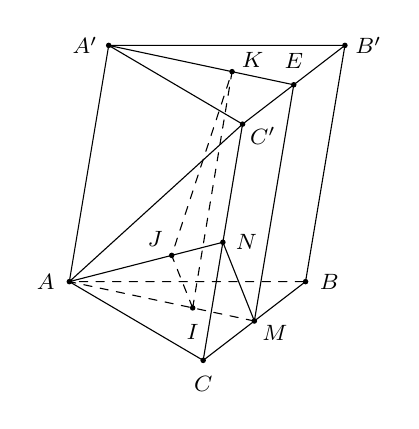
\begin{tikzpicture}[scale=1, font=\footnotesize, line join=round, line cap=round,>=stealth]
\path (0,0)coordinate (A) (3,0) coordinate (B) (1.7,-1) coordinate (C) (0.5,3) coordinate (h);
\foreach \p in {A,B,C} {\draw (\p)--(\p)--+(h) coordinate (\p');}
\draw (A')--(B')--(C')--cycle (A)--(C)--(B);
\path (barycentric cs:A=1,B=1,C=1) coordinate (I) (barycentric cs:A=1,C=1,C'=1) coordinate (J) (barycentric cs:A'=1,B'=1,C'=1) coordinate (K) (barycentric cs:B=1,C=1) coordinate (M) (barycentric cs:C'=1,C=1) coordinate (N) (barycentric cs:B'=1,C'=1) coordinate (E);
\draw[dashed] (M)--(A)--(B) (I)--(J)--(K)--cycle;
\draw (A')--(E)--(M)--(N)--(A)--(C');
\foreach \p/\g in {A/180,C/-90,B/0,A'/180,C'/-30,B'/0,I/-90,J/135,K/30,M/-30,N/0,E/90} \fill[black] (\p) circle(1pt)+(\g:0.3) node{$\p$};
\end{tikzpicture}}
}
\end{ex}

\begin{ex}%[1H4H5-1]
Cho hình lăng trụ $ABC.A'B'C'$. Cắt hình lăng trụ bởi một mặt phẳng ta được một thiết diện. Thiết diện này có tối đa bao nhiêu cạnh?
\choice
{\True $5$}
{$4$}
{$3$}
{$6$}
\loigiai{
Hình lăng trụ $ABC.A'B'C'$ có tất cả $5$ mặt. Do đó một phẳng cắt hình lăng trụ $ABC.A'B'C'$ theo một thiết diện là hình đa giác có nhiều nhất là $5$ cạnh.
}
\end{ex}

\begin{ex}%[1H4V4-4]
Cho tứ diện đều $ABCD$. Gọi $I$ là trung điểm đoạn $CD$, $M$ là điểm nằm trên đoạn $BD$ ($M$ khác $B$ và $D$), $(\alpha)$ là mặt phẳng qua $M$ và song song với mặt phẳng $(ABI)$. Khi đó thiết diện của tứ diện $ABCD$ khi cắt bởi $(\alpha)$ là
\choice
{một tam giác vuông cân}
{một tam giác đều}
{một hình bình hành}
{\True một tam giác cân}
\loigiai{
\immini{Gọi $N$, $P$ lần lượt là giao điểm của $(\alpha)$ với $AD$  và $CD$.\\
Khi đó, thiết diện của tứ diện $ABCD$ và mặt phẳng $(\alpha)$ là tam giác $MNP$.\\
Ta có $(\alpha)\cap (ACD)=NP$, $(ABI)\cap (ACD)=AI$ và $(\alpha)\parallel (ABI)$ nên $NP\parallel AI\Rightarrow\dfrac{NP}{AI}=\dfrac{DP}{DI}$.\hfill $(1)$\\
Tương tự $\dfrac{MP}{BI}=\dfrac{DP}{DI}$.\hfill $(2)$\\
Vì $ABCD$ là tứ diện đều nên $AI=BI$.\hfill $(3)$\\
Từ $(1)$, $(2)$ và $(3)$ suy ra $NP=MP$.\\
Vậy thiết diện là tam giác cân tại $P$.}{\begin{tikzpicture}[scale=1, font=\footnotesize, line join=round, line cap=round,>=stealth]
\def\k{0.4};
\path (0,0)coordinate (B) (4,0) coordinate (D) (1,-1) coordinate (C) ($(C)!0.5!(D)$) coordinate (I) ($(B)!2/3!(I)$) coordinate (G) ($(G)+(0,3)$) coordinate (A) ($(B)!{\k}!(D)$) coordinate (M) ($(A)!{\k}!(D)$) coordinate (N) ($(I)!{\k}!(D)$) coordinate (P);
\draw (A)--(B)--(C)--(D)--cycle (I)--(A)--(C) (N)--(P);
\draw[dashed] (I)--(B)--(D) (N)--(M)--(P);
\foreach \p/\g in {B/180,C/-90,D/0,A/90,I/-90,M/120,P/-30,N/45} \fill[black] (\p) circle(1pt)+(\g:0.3) node{$\p$};
\end{tikzpicture}}}
\end{ex}

\begin{ex}%[1H4V4-5]
Cho hình chóp $S.ABCD$ có đáy $ABCD$ là hình bình hành, mặt bên $SBC$ là tam giác đều. Gọi $M$ là điểm di động trên đoạn thẳng $AB$, $M\ne A;M\ne B$. Qua $M$ dựng mặt phẳng $(\alpha)$ song song với mặt phẳng $(SBC)$. Thiết diện tạo với mặt phẳng $(\alpha)$ và hình chóp $S.ABCD$ là hình gì?
\choice
{\True Hình thang cân}
{Hình thang vuông}
{Hình tam giác}
{Hình bình hành}
\loigiai{
\immini{Ta có $(ABCD)\cap (SBC)=BC$, $M\in (\alpha)\cap (ABCD)$ và $(\alpha)\parallel (SBC)$ nên giao tuyến của $(\alpha)$ và $(ABCD)$ là đường thẳng đi qua $M$ và song song với $BC$, cắt $DC$ tại $N$.\\
Tương tự,
\begin{itemize}
\item giao tuyến của $(\alpha)$ và $(SAB)$ là đường thẳng đi qua $M$ và song song với $SB$, cắt $SA$ tại $Q$;
\item giao tuyến của $(\alpha)$ và $(SCD)$ là đường chứa $N$ và song song với $SC$, cắt $SD$ tại $P$.
\end{itemize} 
}{\begin{tikzpicture}[scale=1, font=\footnotesize, line join=round, line cap=round,>=stealth]
\def\k{0.6};
\path (0,0)coordinate (D)++(3,0) coordinate (C)++(1.1,1) coordinate (B) ($(B)+(D)-(C)$) coordinate (A) (0.7,2.5) coordinate (h) ($(A)+(h)$) coordinate (S) ($(A)!{\k}!(B)$) coordinate (M) ($(D)!{\k}!(C)$) coordinate (N) ($(A)!{\k}!(S)$) coordinate (Q) ($(D)!{\k}!(S)$) coordinate (P);
\draw (S)--(D)--(C)--(B)--cycle (S)--(C) (P)--(N);
\draw[dashed] (S)--(A)--(D) (A)--(B) (P)--(Q)--(M)--(N);
\foreach \p/\g in {A/150,D/240,C/-60, B/0, S/90,M/45,N/-90,P/120,Q/0} \fill[black] (\p) circle(1pt)+(\g:0.3) node{$\p$};
\end{tikzpicture}}\noindent\\
Khi đó, thiết diện là hình thang $MNPQ$.\\
Ta có $(\alpha)\cap (SAD)=PQ$, $(\alpha)\cap (ABCD)=MN$, $(SAD)\cap (ABCD)=AD$ và $MN\parallel BC\parallel AD$ nên $PQ\parallel MN$.\\
Suy ra $MNPQ$ là hình thang.\\
Dễ thấy được $\dfrac{PN}{SC}=\dfrac{DN}{DC}=\dfrac{AM}{AB}=\dfrac{QM}{SB}$.\\
Hơn nữa, tam giác $SBC$ đều nên $SB=SC$. Do đó $MQ=NP$.\\
Vậy $MNPQ$ là hình thang cân.
}
\end{ex}

\begin{ex}%[1H4V4-4]
Cho hình chóp $S.ABC$có đáy là tam giác $ABC$ thỏa mãn $AB=AC=2\sqrt{3}$, $\widehat{BAC}=30^\circ$. Mặt phẳng $(P)$ song song với $(ABC)$ cắt đoạn $SA$ tại $M$ sao cho $SA=3AM$. Thiết diện của mặt phẳng $(P)$ và hình chóp $S.ABC$ có diện tích bằng
\choice
{$\dfrac{4}{9}$}
{\True $\dfrac{4}{3}$}
{$\dfrac{13}{3}$}
{$1$}
\loigiai{
\immini{Gọi $N$, $K$ lần lượt là giao điểm của mặt phẳng $(P)$ và các cạnh $SB$ và $SC$.\\
Khi đó thiết diện của mặt phẳng $(P)$ và hình chóp $S.ABC$ là tam giác $MNK$.\\
Ta có $(P)\cap (SAB)=MN$, $(ABC)\cap (SAB)=AB$ và  $(P)\parallel (ABC)$ nên  $$MN\parallel AB\Rightarrow\dfrac{MN}{AB}=\dfrac{SM}{SA}=\dfrac{2}{3}\Rightarrow MN=\dfrac{2}{3}AB.$$
}{\begin{tikzpicture}[scale=1, font=\footnotesize, line join=round, line cap=round,>=stealth]
\path (0,0)coordinate (A) (4,0) coordinate (C) (1,-1) coordinate (B) ($(A)+(1.5,2.5)$) coordinate (S) (barycentric cs:S=1,A=2) coordinate (M) (barycentric cs:S=1,B=2) coordinate (N) (barycentric cs:S=1,C=2) coordinate (K);
\draw (S)--(A)--(B)--(C)--cycle (S)--(B) (M)--(N)--(K);
\draw[dashed] (A)--(C) (M)--(K);
\foreach \p/\g in {A/180,B/-90,C/0,S/90,M/120,N/180,K/45} \fill[black] (\p) circle(1pt)+(\g:0.3) node{$\p$};
\end{tikzpicture}}\noindent
Tương tự, $MK=\dfrac{2}{3}AC$.\\
Do $MN\parallel AB$ và $MK\parallel AC$ nên $\widehat{NMK}=\widehat{BAC}=30^\circ$.\\
Vậy diện tích tam giác $MNK$ là $$S_{MNK}=\dfrac{1}{2}\cdot MN\cdot MK\cdot\sin\widehat{NMK}=\dfrac{1}{2}\cdot\dfrac{2}{3}AB\cdot\dfrac{2}{3}AC\cdot\sin 30^\circ=\dfrac{4}{3}.$$
}
\end{ex}
\Closesolutionfile{ans}
\indapan{6}{ans/ans-1-C4-B4-De1}
\cauds
\Opensolutionfile{ans}[ans/ans-1-C4-B4-De1-DS]
\begin{ex}%[1H4H4-1]
Cho biết tính đúng sai của mỗi phát biểu sau?
\choiceTF 
{\True Hai mặt phẳng phân biệt không cắt nhau thì song song}
{Nếu mặt phẳng này chứa hai đường thẳng cùng song song với mặt phẳng kia thì hai mặt phẳng đó song song với nhau}
{Hai mặt phẳng cùng song song với mặt phẳng thứ ba thì song song với nhau}
{Hai mặt phẳng phân biệt cùng song song với một đường thẳng thì song song với nhau}
\loigiai{
\begin{itemchoice}
\itemch Đúng.
\itemch Sai. Vì trong giả thiết đã thiếu đi một yếu tố cần thiết là hai đường thẳng phải cắt nhau, khi đó ta mới kết luận hai mặt phẳng song song với nhau.
\itemch Sai. Vì hai mặt phẳng cùng song song với mặt phẳng thứ ba thì chúng vẫn có thể trùng nhau.
\itemch Sai. Vì hai mặt phẳng phân biệt cùng song song với một đường thẳng thì chúng có thể cắt nhau hoặc song song với nhau.
\end{itemchoice}
}
\end{ex}

\begin{ex}%[1H4V4-2]
Cho hình chóp $S.ABCD$ có đáy $ABCD$ là hình bình hành. Gọi $H$, $I$, $K$ lần lượt là trung điểm của $SA$, $SB$, $SC$. Gọi $M$ là giao điểm của $AI$ và $KD$, $N$ là giao điểm của $DH$ và $CI$. Xét tính đúng sai của các khẳng định sau.
\choiceTF
{\True $HI\parallel (ABCD)$}
{\True $(HIK) \parallel (ABCD)$}
{$SM$ và $HI$ chéo nhau}
{$(SMN)$ cắt $(HIK)$}
\loigiai{
\begin{center}
\begin{tikzpicture}[scale=1, font=\footnotesize, line join=round, line cap=round,>=stealth]
\path (0,0)coordinate (D)++(4,0) coordinate (C)++(1,1.5) coordinate (B) ($(B)+(D)-(C)$) coordinate (A) (-0.5,2.5) coordinate (h) ($(A)+(h)$) coordinate (S) (barycentric cs:S=1,A=1) coordinate (H) (barycentric cs:S=1,B=1) coordinate (I) (barycentric cs:S=1,C=1) coordinate (K) (intersection of A--I and K--D) coordinate (M) (intersection of C--I and H--D) coordinate (N);
\draw (S)--(D)--(C)--(B)--(I) (S)--(C)--(I) (D)--(M)--(N)--(S)--(M);
\draw[dashed] (I)--(S)--(A)--(D)--(N) (A)--(B) (I)--(K)--(H)--(I)--(N) (A)--(M);
\foreach \p/\g in {A/150,D/240,C/-60, B/0, S/120,H/180,I/90,K/0,M/0,N/90} \fill[black] (\p) circle(1pt)+(\g:0.3) node{$\p$};
\end{tikzpicture}
\end{center}
\begin{itemchoice}
\itemch Đúng. Ta có $HI\parallel AB\Rightarrow HI\parallel (ABCD)$.
\itemch Đúng. Ta có $HI\parallel AB\Rightarrow HI\parallel (ABCD)$.\\
Tương tự, $KI\parallel BC\Rightarrow KI\parallel (ABCD)$.\\
Suy ra $(HIK)\parallel (ABCD)$.
\itemch Sai. Ta có $\heva{& (SAB)\cap (SDC)=SM \\ & (SAB)\cap (ABCD)=AB\\ &(SCD)\cap (ABCD)=CD\\ & AB\parallel CD}\Rightarrow SM\parallel AB$.\\
Mặt khác $HI\parallel AB$ nên $SM\parallel HI$.
\itemch Sai. Ta có $\heva{& (SAB)\cap (SDC)=SM \\ & (SAB)\cap (ABCD)=AB\\ &(SCD)\cap (ABCD)=CD\\ & AB\parallel CD}\Rightarrow SM\parallel AB$.\\
Mặt khác $HI\parallel AB$ nên $SM\parallel HI$.\\
Chứng minh tương tự ta có $SN\parallel KI$.\\
Do đó $(SMN)\parallel (HIK)$.
\end{itemchoice}
}
\end{ex}

\begin{ex}%[1H4V5-3]
Cho hình hộp $ABCD.A'B'C'D'$. Gọi $G_1$, $G_2$ là trọng tâm của các tam giác $A'BD$, $B'D'C$. Xét tính đúng sai của các mệnh đề sau.
\choiceTF 
{\True $A'D'CB$ là hình bình hành}
{\True $\left(A'BD\right)\parallel\left(B'D'C\right)$}
{\True $G_1, G_2$ cùng thuộc $A C'$}
{$G_1G_2=\dfrac{2}{3}AC'$}
\loigiai{
\begin{center}
\begin{tikzpicture}[scale=1, font=\footnotesize, line join=round, line cap=round,>=stealth]
\path (-0.8,3.5) coordinate (h) (0,0)coordinate (B)++(4,0) coordinate (A)++(0.6,1.5) coordinate (D) ($(B)+(D)-(A)$) coordinate (C);
\foreach \p in {A,B,C,D}\path ($(\p)+(h)$) coordinate (\p');
\path (barycentric cs:A'=1,B=1,D=1) coordinate (G_1) (barycentric cs:B'=1,D'=1,C=1) coordinate (G_2) (barycentric cs:B=1,D=1) coordinate (E) (barycentric cs:B'=1,D'=1) coordinate (E') (barycentric cs:B=1,D'=1) coordinate (O);
\draw (C')--(B')--(B)--(A)--(D)--(D')--cycle (B')--(A')--(D')--(B') (A)--(A')--(D) (B)--(A');
\draw[dashed] (B)--(C)--(D)--(B) (B')--(C)--(C')--(A) (D')--(C)--(E') (A')--(C') (A)--(C)--(A')--(E);
\foreach \p/\g in {C/180,B/240,A/-60,D/0,C'/90,B'/180,A'/0,D'/45,G_1/0,G_2/0,E/-90,E'/90,O/-90} \fill[black] (\p) circle(1pt)+(\g:0.3) node{$\p$};
\end{tikzpicture}
\end{center}
\begin{itemchoice}
\itemch Đúng. Ta có $A'D'\parallel AD\parallel BC$ và $A'D'=AD=BC$ nên $A'D'CB$ là hình bình hành.
\itemch Đúng. Ta có $A'D'BC$ là hình bình hành nên $A'B\parallel CD'\Rightarrow A'B\parallel (B'D'C)$.\\
Dễ thấy $BDD'B'$ là hình bình hành nên $BD\parallel B'D'\Rightarrow BD\parallel (B'D'C)$.\\
Suy ra $(A'BD)\parallel (B'D'C)$.
\itemch Đúng. Gọi $E$, $E'$, $O$ lần lượt là tâm của hình bình hành $ABCD$, $A'B'C'D'$ và hình hộp $ABCD.A'B'C'D'$.\\
Ta có $G_1$ là trọng tâm của tam giác $A'BD$ nên $\dfrac{A'G_1}{A'E}=\dfrac{2}{3}$. Suy ra $G_1$ cũng là trọng tâm của tam giác $A'CA$. Do đó, $G_1\in AO$.\\
Tương tự, $G_2\in C'O$.\\
Vậy $G_1$, $G_2$ cùng thuộc $AC'$.
\itemch Sai. Ta có $G_1O=\dfrac{1}{3}AO=\dfrac{1}{6}AC'$.\\
Tương tự, $G_2O=\dfrac{1}{6}AC'$.\\
Vậy $G_1G_2=G_1O+G_2O=\dfrac{1}{3}AC'$.
\end{itemchoice}
}
\end{ex}

\begin{ex}%[1H4V4-6]
Cho hai hình bình hành $ABCD$ và $ABEF$ nằm ở hai mặt phẳng khác nhau. Gọi $M$ là trọng tâm $\triangle ABE$. Gọi $(P)$ là mặt phẳng đi qua $M$ và song song với mặt $(ADF)$. Lấy $N$ là giao điểm của $(P)$ và $AC$. Xét tính đúng sai của các mệnh đề sau.
\choiceTF 
{$EFDC$ là hình thang}
{\True $FD\parallel EC$}
{\True $(ADF) \parallel (BCE)$}
{$\dfrac{AN}{NC}=3$}
\loigiai{
\begin{center}
\begin{tikzpicture}[scale=1, font=\footnotesize, line join=round, line cap=round,>=stealth]
\path (0,0)coordinate (B)++(3,0) coordinate (C)++(40:2.5) coordinate (D) ($(B)+(D)-(C)$) coordinate (A)++(80:2) coordinate (F) ($(F)+(B)-(A)$) coordinate (E) (barycentric cs:A=1,B=1,E=1) coordinate (M) (barycentric cs:A=1,B=2) coordinate (K) (barycentric cs:E=1,B=1) coordinate (I) (barycentric cs:A=1,C=2) coordinate (N);
\draw (B)--(C)--(D)--(F)--(E)--cycle (C)--(E)--(B);
\draw[dashed] (B)--(A)--(D) (F)--(A)--(E) (I)--(A)--(C) (M)--(K)--(N);
\foreach \p/\g in {A/45,B/-120,C/-30,D/0,F/90,E/120,M/135,K/-90,I/180,N/45} \fill[black] (\p) circle(1pt)+(\g:0.3) node{$\p$};
\end{tikzpicture}
\end{center}
\begin{itemchoice}
\itemch Sai. Ta có $EF\parallel AB\parallel CD$ và $EF=AB=CD$ nên $EFDC$ là hình bình hành.
\itemch Đúng. Vì $EFDC$ là hình bình hành nên $FD\parallel EC$.
\itemch Đúng. Ta có $FD\parallel EC\Rightarrow FD\parallel (BCE)$.\\
Tương tự, $AD\parallel BC\Rightarrow AD\parallel (BCE)$.\\
Suy ra $(ADF)\parallel (BCE)$.
\itemch Sai. Gọi $I$ là trung điểm của $EB$ và $K$ là giao điểm của $(P)$ với đường thẳng $AB$.\\
Ta có $(P)\parallel (ADF)\parallel (BCE)$, $(P)\cap (ABEF)=MK$ và $(BEC)\cap (ABEF)=BE$ nên $MK\parallel AB$.\\
Suy ra $\dfrac{AK}{AB}=\dfrac{AM}{AI}=\dfrac{2}{3}\Rightarrow \dfrac{AK}{KB}=2$.\\
Ta có $(P)\parallel (ADF)\parallel (BCE)$, $(P)\cap (ABCD)=NK$ và $(BEC)\cap (ABCD)=BC$ nên $NK\parallel BC$.\\
Do đó, $\dfrac{AN}{NC}=\dfrac{AK}{KB}=2$.
\end{itemchoice}
}
\end{ex}

\Closesolutionfile{ans}
\indapan{3}{ans/ans-1-C4-B4-De1-DS}

\Opensolutionfile{ans}[ans/ans-1-C4-B4-De1-KQ]
\caukq
\begin{ex}%[1H4N5-1]
Trong hình hộp $ABCD.A'B'C'D'$, các đường thẳng $AC'$, $BD'$, $CA'$ cùng đi qua điểm $I$. Tính tỉ số  $\dfrac{IB'}{ID}$.
\shortans{$1$}
\loigiai{
\immini{Trong hình hộp, các đường chéo $AC'$, $BD'$, $CA'$ và $DB'$ đồng quy tại tâm $I$ là trung điểm của mỗi đường.\\
Vậy $\dfrac{IB'}{ID}=1$.}{\begin{tikzpicture}[scale=1, font=\footnotesize, line join=round, line cap=round,>=stealth]
\path (-0.7,2.5) coordinate (h) (0,0)coordinate (B)++(2.2,0) coordinate (C)++(1,0.8) coordinate (D) ($(B)+(D)-(C)$) coordinate (A);
\foreach \p in {A,B,C,D}\path ($(\p)+(h)$) coordinate (\p');
\path (barycentric cs:A=1,C'=1) coordinate (I);
\draw (A')--(B')--(B)--(C)--(D)--(D')--cycle (B')--(C')--(D') (C)--(C');
\draw[dashed] (D')--(B)--(A)--(D)--(B') (C')--(A)--(A')--(C);
\foreach \p/\g in {A/45,B/240,C/-60,D/0,A'/90,B'/180,C'/90,D'/45,I/10} \fill[black] (\p) circle(1pt)+(\g:0.3) node{$\p$};
\end{tikzpicture}}
}
\end{ex}

\begin{ex}%[1H4H4-5]
Cho hình chóp $S.ABCD$ có đáy $ABCD$ là hình thang với $AD$ là đáy lớn và $AD=2BC$. Gọi $M$, $N$ lần lượt là trung điểm của $SA$ và $AD$. Biết mặt phẳng $(\alpha)$ đi qua $MN$ và song song với $(SCD)$ cắt cạnh $BC$ tại điểm $E$. Tính tỉ số $\dfrac{CE}{CB}$.
\shortans{$\dfrac{CE}{CB}=1$} 
\loigiai{
\immini{Ta có $(\alpha)\cap (ABCD)=NE$, $(SCD)\cap (ABCD)=CD$ và $(\alpha)\parallel (SCD)$ nên $NE\parallel CD$.\\
Theo đề bài thì $ND\parallel BC$.\\
Do đó $NECD$ là hình bình hành. Suy ra $$CE=ND=\dfrac{1}{2}AD=BC.$$
 Vậy $E\equiv B$ và $\dfrac{CE}{CB}=1$.
}{\begin{tikzpicture}[scale=1, font=\footnotesize, line join=round, line cap=round,>=stealth]
\path (0,0)coordinate (B)++(2,0) coordinate (C)++(1.3,1) coordinate (D) ($(B)+(D)-(C)$) coordinate (a) (barycentric cs:a=-2,D=1) coordinate (A) (1,2.5) coordinate (h) ($(A)+(h)$) coordinate (S) (barycentric cs:S=1,A=1) coordinate (M) (barycentric cs:D=1,A=1) coordinate (N);
\draw (S)--(A)--(B)--(C)--(D)--cycle (M)--(B)--(S)--(C);
\draw[dashed] (A)--(D) (M)--(N)--(B);
\foreach \p/\g in {A/150,B/240,C/-60, D/0, S/90,M/150,N/-90} \fill[black] (\p) circle(1pt)+(\g:0.3) node{$\p$};
\end{tikzpicture}}
} 
\end{ex}

\begin{ex}%[1H4H4-6]
Cho hình chóp $S.ABCD$ có đáy $ABCD$ là hình bình hành tâm $O$. Gọi $M$, $N$ lần lượt là trung điểm của $SA$ và $SD$. Tính tỉ số diện tích $\dfrac{S_{\triangle SBC}}{S_{\triangle ONN}}$.
\shortans{$\dfrac{S_{\triangle SBC}}{S_{\triangle ONN}}=4$} 
\loigiai{
\immini{Ta có $OM$, $ON$ lần lượt là đường trung bình của tam giác $SAC$ và $SBD$ nên $SC\parallel OM$, $SC=2OM$ và $SB\parallel ON$, $SB=2ON$.\\
Do đó, $$\dfrac{S_{\triangle SBC}}{S_{\triangle OMN}}=\dfrac{\tfrac{1}{2}\cdot SB\cdot SC\cdot\sin\widehat{BSC}}{\tfrac{1}{2}\cdot ON\cdot OM\cdot\widehat{NOM}}=\dfrac{SB}{ON}\cdot\dfrac{SC}{OM}=4.$$}{\begin{tikzpicture}[scale=1, font=\footnotesize, line join=round, line cap=round,>=stealth]
\path (0,0)coordinate (B)++(3,0) coordinate (C)++(1.5,1) coordinate (D) ($(B)+(D)-(C)$) coordinate (A) (0.5,2.5) coordinate (h) ($(A)+(h)$) coordinate (S) (barycentric cs:S=1,A=1) coordinate (M) (barycentric cs:S=1,D=1) coordinate (N) (barycentric cs:C=1,A=1) coordinate (O);
\draw (S)--(B)--(C)--(D)--cycle (S)--(C);
\draw[dashed] (S)--(A)--(B)--(D)--(A)--(C) (O)--(M)--(N)--cycle;
\foreach \p/\g in {A/150,B/240,C/-60, D/0, S/90,M/180,N/30,O/-90} \fill[black] (\p) circle(1pt)+(\g:0.3) node{$\p$};
\end{tikzpicture}}
} 
\end{ex}

\begin{ex}%[1H4V4-3]
Cho hình chóp $S.ABCD$, có đáy $ABCD$ là hình bình hành tâm $O$. Gọi $M$, $N$, $E$ lần lượt là trung điểm của $SA$, $SD$ và $AB$.
Gọi $F$ là một điểm thuộc $ON$. Đường thẳng $AF$ cắt mặt phẳng $(SBC)$ tại $G$. Tính tỉ số $\dfrac{AF}{AG}$.
\shortans{$\dfrac{AF}{AG}=0{,}5$}
\loigiai{
\immini{Ta có $MN$ là đường trung bình của tam giác $SAD$ nên $MN\parallel AD\parallel BC\Rightarrow MN\parallel (SBC)$.\\
Tương tự, $ME\parallel (SBC)$.\\
Suy ra $(MNE)\parallel (SBC)$.\\
Ta có $OE$ cũng là đường trung bình của tam giác $ABD$ nên $OE\parallel AD\parallel MN$. Do đó $OE\subset (MNE)$ hay $(MNE)\equiv (MNOE)$.
}{\begin{tikzpicture}[scale=1, font=\footnotesize, line join=round, line cap=round,>=stealth]
\path (0,0)coordinate (B)++(3,0) coordinate (C)++(1.5,1) coordinate (D) ($(B)+(D)-(C)$) coordinate (A) (-0.5,2.5) coordinate (h) ($(A)+(h)$) coordinate (S) (barycentric cs:S=1,A=1) coordinate (M) (barycentric cs:S=1,D=1) coordinate (N) (barycentric cs:B=1,A=1) coordinate (E) (barycentric cs:C=1,A=1) coordinate (O) ($(O)!0.6!(N)$) coordinate (F);
\draw (S)--(B)--(C)--(D)--cycle (S)--(C);
\draw[dashed] (S)--(A)--(B) (C)--(A)--(D)--(B) (M)--(N)--(O)--(E)--(M);
\foreach \p/\g in {A/150,B/240,C/-60, D/0, S/90,M/150,N/30,E/150,F/0,O/-90} \fill[black] (\p) circle(1pt)+(\g:0.3) node{$\p$};
\end{tikzpicture}}\noindent
Như thế $EF\subset (MNOE)\parallel (SBC)$ nên $EF\parallel (SBC)$.\\
Ta có $(AEF)\cap (SBC)=BG$ nên $EF\parallel BG\Rightarrow\dfrac{AF}{AG}=\dfrac{AE}{AB}=0{,}5$.
}
\end{ex}

\begin{ex}%[1H4V4-6]
Cho hình chóp $S.ABC$ có $D$, $E$, $F$ lần lượt là trọng tâm các tam giác $SAB$, $SBC$, $SCA$. Tam giác $ABC$ có diện tích bằng $2025$ cm$^2$. Mặt phẳng $(DEF)$ cắt các cạnh $SA$, $SB$, $SC$ lần lượt tại $A'$, $B'$, $C'$. Tính diện tích tam giác $A'B'C'$.
\shortans{$S_{\triangle A'B'C'}=900$ cm$^2$} 
\loigiai{
\immini{Gọi $M$, $N$, $P$ lần lượt là trung điểm của $AB$, $BC$, $CA$.\\
Ta có $\dfrac{SD}{SM}=\dfrac{1}{3}=\dfrac{SE}{SN}\Rightarrow DE\parallel MN$. Mà $MN\subset (ABC)$ nên $DE\parallel (ABC)$.\\
Tương tự, $DF\parallel (ABC)$.\\
Suy ra $(DEF)\parallel (ABC)$.\\
Ta có $(DEF)\equiv (A'B'C')$ nên $(A'B'C')\parallel (ABC)$.\\
Dễ thấy $A'B'\parallel AB$ nên $\dfrac{A'B'}{AB}=\dfrac{SD}{SM}=\dfrac{2}{3}$.\\
Tương tự $\dfrac{A'C'}{AC}=\dfrac{2}{3}$.}{\begin{tikzpicture}[scale=1, font=\footnotesize, line join=round, line cap=round,>=stealth]
\path (0,0)coordinate (A) (4,0) coordinate (C) (1,-1) coordinate (B) ($(A)+(1.5,2.5)$) coordinate (S) (barycentric cs:S=1,A=2) coordinate (A') (barycentric cs:S=1,B=2) coordinate (B') (barycentric cs:S=1,C=2) coordinate (C') (barycentric cs:S=1,A=1,B=1) coordinate (D) (barycentric cs:S=1,B=1,C=1) coordinate (E) (barycentric cs:S=1,A=1,C=1) coordinate (F) (barycentric cs:A=1,B=1) coordinate (M) (barycentric cs:C=1,B=1) coordinate (N) (barycentric cs:A=1,C=1) coordinate (P);
\draw (S)--(A)--(B)--(C)--cycle (M)--(S)--(B) (N)--(S) (A')--(B')--(C');
\draw[dashed] (A)--(C) (S)--(P) (A')--(C');
\foreach \p/\g in {A/180,B/-90,C/0,S/90,A'/150,B'/45,C'/30,D/210,E/-30,F/135,M/-120,N/-60,P/-90} \fill[black] (\p) circle(1pt)+(\g:0.3) node{$\p$};
\end{tikzpicture}}\noindent
Ta có $\dfrac{S_{\triangle A'B'C'}}{S_{\triangle ABC}}=\dfrac{\tfrac{1}{2}\cdot A'B'\cdot A'C'\cdot\sin\widehat{B'A'C'}}{\tfrac{1}{2}\cdot AB\cdot AC\cdot\sin\widehat{BAC}}=\dfrac{A'B'}{AB}\cdot\dfrac{A'C'}{AC}=\dfrac{4}{9}$.\\
Vậy $S_{\triangle A'B'C'}=\dfrac{4}{9}\cdot S_{\triangle ABC}=\dfrac{4}{9}\cdot 2025=900$ cm$^2$.
} 
\end{ex}

\begin{ex}%[1H4C4-6]
Cho hình hộp $ABCD.A'B'C'D'$ có $M$, $N$, $P$ lần lượt là trung điểm của $A'B'$, $BC$, $DD'$. Gọi $E$, $F$, $G$ lần lượt là giao điểm của $AC'$ với các mặt phẳng $(A'BD)$, $(MNP)$, $(CB'D')$. Tính tỉ số $\dfrac{EG}{EF}$.
\shortans{$\dfrac{EG}{EF}=2$} 
\loigiai{
\immini{Gọi $H$, $I$ lần lượt là trung điểm của $B'C$ và $B'D$.\\ 
Ta có $HN$ là đường trung bình của tam giác $CBB'$ nên $HN\parallel BB'\parallel DD'$ và $$HN=\dfrac{1}{2}BB'=\dfrac{1}{2}DD'=D'P.$$
Suy ra $PNHD'$ là hình bình hành. Do đó $$PN\parallel D'H\Rightarrow PN\parallel (CB'D').$$}{\begin{tikzpicture}[scale=1, font=\footnotesize, line join=round, line cap=round,>=stealth]
\path (-0.8,3) coordinate (h) (0,0)coordinate (D)++(3.5,0) coordinate (C)++(1.3,1) coordinate (B) ($(D)+(B)-(C)$) coordinate (A);
\foreach \p in {A,B,C,D}\path ($(\p)+(h)$) coordinate (\p');
\path (barycentric cs:A'=1,B'=1) coordinate (M) (barycentric cs:C=1,B=1) coordinate (N) (barycentric cs:D=1,D'=1) coordinate (P) (barycentric cs:C=1,B'=1) coordinate (H) (barycentric cs:B'=1,D'=1) coordinate (I);
\draw (A')--(D')--(D)--(C)--(B)--(B')--cycle (B')--(D')--(C')--(B')--(C)--(C') (D')--(C) (H)--(N);
\draw[dashed] (D)--(A)--(B) (C')--(A)--(A')  (M)--(N)--(P)--(M) (D')--(H) (C)--(I);
\foreach \p/\g in {A/180,D/240,C/-60,B/0,A'/90,D'/180,C'/135,B'/45,M/90,N/-30,P/180,H/30,I/90} \fill[black] (\p) circle(1pt)+(\g:0.3) node{$\p$};
\end{tikzpicture}}\noindent
Chứng minh tương tự, $MN\parallel (CB'D')$.\\
Do đó $(MNP)\parallel (CB'D')$.\\
Ta cũng chứng minh được $(MNP)\parallel (A'BD)$.\\
Ba mặt phẳng $(A'BD)$, $(MNP)$, $(CB'D')$ song song với nhau nên chắn trên các đường thẳng $A'B'$ và $AC'$ những đoạn thẳng tương ứng tỉ lệ. Tức là $$\dfrac{EG}{A'B'}=\dfrac{EF}{A'M}\Rightarrow\dfrac{EG}{EF}=\dfrac{A'B'}{A'M}=2.$$
} 
\end{ex}
\Closesolutionfile{ans}
\indapan{6}{ans/ans-1-C4-B4-De1-KQ}
\subsection{Đề số 2}

\Opensolutionfile{ans}[ans/ans-1-C4-B4-De2]
\caulc

\begin{ex}%[1H4N5-1]
	Cho hình hộp $ABCD.A'B'C'D'$. Mệnh đề nào sau đây \textbf{sai}?
	\choice
	{$\left(BA'C'\right)\parallel\left(ACD'\right)$}
	{$\left(ADD'A'\right)\parallel\left(BCC'B'\right)$}
	{$\left(BA'D\right)\parallel\left(CB'D'\right)$}
	{\True $(ABA')\parallel(CB'D')$}
	\loigiai{
		\begin{center}
			\begin{tikzpicture}[scale=0.6, font=\footnotesize, line join=round, line cap=round, >=stealth]
				\def\bc{4} % cạnh BC
				\def\ba{2} % cạnh BA
				\def\h{4} % đường cao
				\def\gocB{35} % góc B của đáy
				\coordinate[label=below left:$B$] (B) at (0,0);
				\coordinate[label=above left:$A$] (A) at (\gocB:\ba);
				\coordinate[label=below:$C$] (C) at (\bc,0);
				\coordinate[label=right:$D$] (D) at ($(C)-(B)+(A)$);
				\coordinate (H) at ($(B)!0.4!(D)$); % Hình chiếu của A'
				\coordinate[label=above left:$A'$] (A') at ($(H)+(90:\h)$);
				\coordinate[label=left:$B'$] (B') at ($(B)-(A)+(A')$);
				\coordinate[label=below right:$C'$] (C') at ($(C)-(A)+(A')$);
				\coordinate[label=right:$D'$] (D') at ($(D)-(A)+(A')$);
				\draw (B')--(B)--(C)--(D)--(D')--(A')--(B')--(C')--(D') (C)--(C');
				\draw[dashed] (A)--(D) (A')--(A)--(B);
				\foreach \diem in {A,B,C,D,A',B',C',D'}	\fill (\diem)circle(1.5pt);
			\end{tikzpicture}
			
		\end{center}
		Ta có\\
		\begin{itemize}
			\item $\heva{& BA'\parallel CD' \\ & A'C'\parallel AC }$$\Rightarrow (BA'C')\parallel(ACD')$.
			\item $\heva{& AD\parallel BC \\ & AA'\parallel BB' }$$\Rightarrow (ADD'A')\parallel(BCC'B')$.
			\item $\heva{& BD\parallel B'D' \\ & A'D\parallel B'C }$$\Rightarrow (BA'D)\parallel(CB'D')$.
		\end{itemize}
		Mặt khác $B'\in (ABA')\cap (CB'D') $ nên D sai.}
\end{ex}
\begin{ex}%[1H4H5-3]
	Cho hình hộp $ABCD.A'B'C'D'$. Mặt phẳng $(AB'D')$ song song với mặt phẳng nào sau đây?
		\choice
	{$(BA'C')$}
	{\True $(C'BD)$}
	{$(BDA')$}
	{$(ACD')$}
	\loigiai{
		\begin{center}
			\begin{tikzpicture}[scale=1, font=\footnotesize, line join=round, line cap=round, >=stealth]
				\def\bc{4} % cạnh BC
				\def\ba{2} % cạnh BA
				\def\h{4} % đường cao
				\def\gocB{45} % góc B của đáy
				\coordinate[label=below left:$B$] (B) at (0,0);
				\coordinate[label=above left:$A$] (A) at (\gocB:\ba);
				\coordinate[label=below:$C$] (C) at (\bc,0);
				\coordinate[label=right:$D$] (D) at ($(C)-(B)+(A)$);
				\coordinate (H) at ($(B)!0.4!(D)$); % Hình chiếu của A'
				\coordinate[label=above left:$A'$] (A') at ($(H)+(90:\h)$);
				\coordinate[label=left:$B'$] (B') at ($(B)-(A)+(A')$);
				\coordinate[label=below right:$C'$] (C') at ($(C)-(A)+(A')$);
				\coordinate[label=right:$D'$] (D') at ($(D)-(A)+(A')$);
				\draw (B')--(B)--(C)--(D)--(D')--(A')--(B')--(C')--(D') (C)--(C');
				\draw[dashed] (C)--(A)--(D)--(B) (A')--(A)--(B) (B')--(A)--(D');
				\foreach \diem in {A,B,C,D,A',B',C',D'}	\fill (\diem)circle(1.5pt);
			\end{tikzpicture}
			
		\end{center}
		Ta có $\heva{&B'D'\parallel BD\\& AD'\parallel C'B}\Rightarrow (AB'D')\parallel(C'BD)$.}
\end{ex}
\begin{ex}%[1H4H4-2]
	Cho hai hình bình hành $ABCD$ và $ABEF$ có tâm lần lượt là $O$ và $O'$, không cùng nằm trong một mặt phẳng. Gọi $M$ là trung điểm $AB$, xét các khẳng định
	\begin{description}
		\item[(I)] $(ADF)\parallel(BCE)$
		\item[(II)] $(MOO')\parallel(ADF)$
		\item[(III)] $(MOO')\parallel(BCE)$
		\item[(IV)] $(ACE)\parallel(BDF)$
	\end{description}
	Những khẳng định nào đúng?
	\choice
	{$(I)$}	
	{$(I),(I)$}
	{\True $(I),(II),(III)$}	
	{$(I),(II),(III),(IV)$}
	\loigiai{
		\begin{center}
				\begin{tikzpicture}[>=stealth,line join=round,line cap=round,font=\footnotesize,scale=1]
				\path (0,0)coordinate[label=left:$A$](A) (4,0)coordinate[label=right:$B$](B) (5,-1)coordinate[label=right:$C$](C) (1,-1)coordinate[label=left:$D$](D) (1,2)coordinate[label=above:$F$](F) (5,2)coordinate[label=above:$E$](E) ;
				\coordinate[label=above left:$M$] (M) at ($(A)!0.5!(B)$);
				\coordinate[label=below:$O$] (O) at ($(D)!0.5!(B)$);
				\coordinate[label=above:$O'$] (O') at ($(F)!0.5!(B)$);
				\draw (C)--(D)--(F)--(E)--cycle (D)--(A)--(F) ;
				\draw[dashed] (A)--(B)--(D) (E)--(B)--(F) (M)--(O)--(O')--cycle (B)--(C);
				\foreach \diem in {A,B,C,D,E,F,M,O,O'} \fill[black](\diem)circle(1.5pt);		
			\end{tikzpicture}
		\end{center}
		Xét hai mặt phẳng $(ADF)$ và $(BCE)$ có  $\heva{& AD\parallel BC \\ & AF\parallel BE }$ nên khẳng định $(I)$: $$(ADF)\parallel(BCE) \text{ là đúng}.$$
		Xét hai mặt phẳng $(ADF)$ và $(MOO')$ có  $\heva{& AD\parallel MO \\ & AF\parallel MO' }$ nên khẳng định $(II)$: $$(MOO')\parallel(ADF) \text{ là đúng}.$$
		Vì $(I)\colon (ADF)\parallel(BCE)$ đúng và $(II)\colon (MOO')\parallel(ADF)$ đúng nên theo tính chất bắc cầu ta có khẳng định $(III)\colon (MOO')\parallel(BCE)$ đúng.\\
		Xét mặt phẳng $(ABCD)$ có $AC\cap BD=O$ nên hai mặt phẳng $(ACE)$ và $(BDF)$ có điểm $O$ chung vì vậy không song song nên khẳng định $(IV)\colon (ACE)\parallel(BDF)$ sai.}
\end{ex}
\begin{ex}%[1H4N5-3]
	Cho hình hộp $ABCD.A'B'C'D'$. Trong các khẳng định sau, khẳng định nào \textbf{sai}?
		\choice
	{$(ABCD) \parallel (A'B'C'D')$}
	{$(AA'D')\parallel (BCC')$}
	{\True $(BDD')\parallel (ACC')$}
	{$(ABB')\parallel (CDC')$}
	\loigiai{
		\begin{center}
			\begin{tikzpicture}[scale=1, font=\footnotesize, line join=round, line cap=round, >=stealth]
				\def\bc{4} % cạnh BC
				\def\ba{2} % cạnh BA
				\def\h{4} % đường cao
				\def\gocB{35} % góc B của đáy
				\coordinate[label=below left:$B$] (B) at (0,0);
				\coordinate[label=above left:$A$] (A) at (\gocB:\ba);
				\coordinate[label=below:$C$] (C) at (\bc,0);
				\coordinate[label=right:$D$] (D) at ($(C)-(B)+(A)$);
				\coordinate (H) at ($(B)!0.4!(D)$); % Hình chiếu của A'
				\coordinate[label=above left:$A'$] (A') at ($(H)+(90:\h)$);
				\coordinate[label=left:$B'$] (B') at ($(B)-(A)+(A')$);
				\coordinate[label=below right:$C'$] (C') at ($(C)-(A)+(A')$);
				\coordinate[label=right:$D'$] (D') at ($(D)-(A)+(A')$);
				\draw (B')--(B)--(C)--(D)--(D')--(A')--(B')--(C')--(D') (C)--(C') (A')--(C') (B')--(D');
				\draw[dashed] (C)--(A)--(D)--(B) (A')--(A)--(B) (A)--(C) (B)--(D);
				\foreach \diem in {A,B,C,D,A',B',C',D'}	\fill (\diem)circle(1.5pt);
			\end{tikzpicture}			
		\end{center}
Khẳng định ``$(BDD')\parallel (ACC')$''	sai vì hai mặt phẳng này có điểm chung là $O$ với $O=AC\cap BD$.

	}
\end{ex}
\begin{ex} % Câu 5:%[Dự án đề theo cấu trúc mới 10,11-NCT]%[1H4V4-2]
	Cho hình lăng trụ $ABC.A'B'C'$. Gọi $I$, $J$, $K$ lần lượt là trọng tâm các tam giác $ABC$, $A'B'C'$, $ACC'$. Mặt phẳng nào sau đây song song với $(IJK)$
		\choice
	{$(ABB')$}
	{$(ACC')$}
	{\True $(BB'C')$}
	{$(ABC')$}
	\loigiai{
		Gọi $M$, $N$, $P$ lần lượt là trung điểm $BC$,$B'C'$ và $CC'$.\\
		Ta có $\heva{& IJ\parallel MN \\ & IJ\not\subset (BB'C) \\ & MN\subset (BB'C) }$ nên $IJ\parallel(BB'C')$.\\
		Ta có $\heva{& JK\parallel NP \\ & JK\not\subset (BB'C) \\ & NP\subset (BB'C) }$ nên $JK\parallel(BB'C')$.\\
		Từ đó suy ra $(IJK)\parallel(BB'C')$.}
\end{ex}
\begin{ex}%[1H4N5-3]
	Cho hình hộp $ABCD.A'B'C'D'$. Gọi $O$, $O'$ lần lượt là tâm của hai đáy $ABCD$ và $A'B'C'D'$. Mệnh đề nào sau đây \textbf{sai}?
		\choice
	{\True $(BA'D')\parallel(ADC')$}
	{$(ABB')\parallel(CDD')$}
	{$(B'AC)\parallel(DA'C')$}
	{$(ABO')\parallel(OC'D')$}
	\loigiai{
		\begin{center}
			\begin{tikzpicture}[scale=1, font=\footnotesize, line join=round, line cap=round, >=stealth]
				\def\bc{4} % cạnh BC
				\def\ba{2} % cạnh BA
				\def\h{4} % đường cao
				\def\gocB{35} % góc B của đáy
				\coordinate[label=below left:$B$] (B) at (0,0);
				\coordinate[label=above left:$A$] (A) at (\gocB:\ba);
				\coordinate[label=below:$C$] (C) at (\bc,0);
				\coordinate[label=right:$D$] (D) at ($(C)-(B)+(A)$);
				\coordinate (H) at ($(B)!0.4!(D)$); % Hình chiếu của A'
				\coordinate[label=above left:$A'$] (A') at ($(H)+(90:\h)$);
				\coordinate[label=left:$B'$] (B') at ($(B)-(A)+(A')$);
				\coordinate[label=below right:$C'$] (C') at ($(C)-(A)+(A')$);
				\coordinate[label=right:$D'$] (D') at ($(D)-(A)+(A')$);
				\coordinate[label=below:$O$] (O) at ($(A)!0.5!(C)$);
				\coordinate[label=above:$O'$] (O') at ($(A')!0.5!(C')$);
				\draw (B')--(B)--(C)--(D)--(D')--(A')--(B')--(C')--(D') (C)--(C') (A')--(C') (B')--(D');
				\draw[dashed] (C)--(A)--(D)--(B) (A')--(A)--(B) (A)--(C) (B)--(D);
				\foreach \diem in {A,B,C,D,A',B',C',D',O,O'}	\fill (\diem)circle(1.5pt);
			\end{tikzpicture}
			
		\end{center}
		Ta thấy $AB'\cap A'B$, mà $(BA'D')\equiv (CBA'D')$ và $(ADC')\equiv (ADC'B')$ nên hai mặt này cắt nhau.}
\end{ex}

	\begin{ex}%[1H4V4-4]
		Cho hình chóp $S.ABCD$ có đáy $ABCD$ là hình bình hành, mặt bên $SBC$ là tam giác đều. Gọi $M$ là điểm di động trên đoạn thẳng $AB$, ($M\ne A;M\ne B$). Qua $M$ dựng mặt phẳng $(\alpha)$ song song với mặt phẳng $(SBC)$. Thiết diện tạo với mặt phẳng $(\alpha)$ và chóp $S.ABCD$ là hình gì?
		\choice
		{\True Hình thang cân}
		{ Hình thang vuông}
		{ Hình tam giác}
		{ Hình bình hành}
		\loigiai{
			\begin{center}
				\begin{tikzpicture}[scale=1, font=\footnotesize, line join=round, line cap=round, >=stealth]
					\def\bc{5} % cạnh BC
					\def\ba{3} % cạnh BA
					\def\h{5} % đường cao
					\def\gocB{30} % góc B của đáy
					\coordinate[label=below left:$B$] (B) at (0,0);
					\coordinate[label=above right:$A$] (A) at (\gocB:\ba);
					\coordinate[label=below:$C$] (C) at (\bc,0);
					\coordinate[label=right:$D$] (D) at ($(C)-(B)+(A)$);
					\coordinate[label=above:$O$] (O) at ($(A)!.5!(C)$);
					\coordinate[label=above:$S$] (S) at ($(O)+(105:\h)$);
					\coordinate[label=left:$M$] (M) at ($(A)!0.7!(B)$);
					\coordinate[label=right:$N$] (N) at ($(D)!0.7!(C)$);
					\coordinate[label=left:$Q$] (Q) at ($(A)!0.7!(S)$);
					\coordinate[label=right:$P$] (P) at ($(D)!0.7!(S)$);
					\draw (B)--(C)--(D)--(S)--cycle (S)--(C) (N)--(P);
					\draw[dashed] (C)--(A)--(D)--(B) (S)--(A)--(B) (P)--(Q)--(M)--(N);
					\foreach \diem in {A,B,C,D,S,O,M,N,P,Q}	\fill (\diem)circle(1.5pt);
				\end{tikzpicture}
				
			\end{center}
			Ta có $\heva{& (\alpha)\parallel (SBC) \\ & (SBC)\cap (ABCD)=BC \\ & (\alpha)\cap (ABCD)=\{ M \} }$. Suy ra $ (\alpha)\cap (ABCD)=MNM $ và $ MN\parallel BC$.\\
			Tương tự $\heva{&(\alpha)\cap (SAB)=MQ\\&MQ\parallel SB\\& (\alpha)\cap (SDC)=NP \\& NP\parallel SC}$.\\ Suy ra
			$(\alpha)\cap (SAD)=PQ$ và $PQ\parallel AD\parallel BC$.\\
			Thiết diện taọ thành là hình thang $MNPQ$ do $SBC$ là tam giác đều nên $MQ=NP$.\\
			Vậy $MNPQ$ là hình thang cân.}
	\end{ex}
	\begin{ex}%[1H4V4-4]
		Cho tứ diện đều $ABCD$. Gọi $I$ là trung điểm đoạn $CD$, $M$ là điểm nằm trên đoạn $BC$ ($M$ khác $B$ và $C$), $(\alpha)$ là mặt phẳng qua $M$ và song song với mặt phẳng $(ABI)$. Khi đó thiết diện của tứ diện $ABCD$ khi cắt bởi $(\alpha)$ là
		\choice
		{ Một tam giác vuông cân}
		{ Một tam giác đều}
		{ Một hình bình hành}
		{\True Một tam giác cân}
		\loigiai{
			\begin{center}
				\begin{tikzpicture}[scale=1, font=\footnotesize, line join=round, line cap=round, >=stealth]
					\def\ac{4} % cạnh AC
					\def\ab{2} % cạnh AB
					\def\h{4} % chiều cao
					\def\gocA{50} % góc A của đáy
					\coordinate[label=left:$A$] (A) at (0,0);
					\coordinate[label=right:$C$] (C) at (\ac,0);
					\coordinate[label=below left:$B$] (B) at (-\gocA:\ab);
					\coordinate(M) at ($(B)!.5!(C)$);
					\coordinate (G) at ($(A)!2/3!(M)$);
					\coordinate[label=above:$D$] (D) at ($(G)+(90:\h)$);
					\coordinate[label=right:$I$] (I) at ($(C)!0.5!(D)$);
					\coordinate[label=below:$M$] (m) at ($(C)!0.7!(B)$);
					\coordinate[label=below:$P$] (P) at ($(C)!0.7!(A)$);
					\coordinate[label=right :$N$] (N) at ($(C)!0.7!(I)$);
					\draw (A)--(B)--(C)--(D)--cycle (D)--(B)--(I) (m)--(N);
					\draw[dashed] (A)--(C) (D) (A)--(I) (m)--(P)--(N);
					\foreach \diem in {A,B,C,D,I,m,N,P}	\fill (\diem)circle(1.5pt);
				\end{tikzpicture}
			\end{center}
		\begin{itemize}
			\item $(ABI)\cap (BCD)=BI$, $(\alpha)$ và $(BCD)$ có điểm $M$ chung. Vậy giao tuyến của $(\alpha)$ và $(BCD)$ là đường thẳng qua $M$ song song với $IB$, giả sử cắt $CD$ tại $N$.
			\item Lập luận tương tự ta được $NP\parallel AI$, $P\in AC$; $PM\parallel AB$.
			\item Do $ABCD$ là tứ diện đều nên tam giác $ABI$ cân tại $I$. Suy ra $ \vartriangle MNP$ cân tại $N$.
		\end{itemize}
		}
	\end{ex}
	\begin{ex}%[1H4V4-2]
		Cho hình chóp $S.ABCD$ đáy là hình thang, $AB\parallel CD$, $AB=a$; $CD=2a$, gọi $I$ là giao điểm của $AC$ và $BD$. Qua $I$ kẻ đường thẳng song song $CD$ cắt $BC$ tại $M$. Trên cạnh $SC$ lấy điểm $N$ sao cho $CN=2NS$ (tham khảo hình vẽ)
		\begin{center}
			\begin{tikzpicture}[scale=1, font=\footnotesize, line join=round, line cap=round, >=stealth]
				\def\ad{4} % cạnh AD
				\def\ab{2} % cạnh AB
				\def\bc{2} % chéo AC
				\def\as{4} % cạnh AS
				\def\gocA{50} % góc A của đáy
				\def\gocB{130} % góc B của đáy
				\coordinate[label=left:$B$] (A) at (0,0);
				\coordinate[label=below left:$A$] (B) at (-\gocA:\ab);
				\coordinate[label=below right:$D$] (C) at ($(B)+(180-\gocA-\gocB:\bc)$);
				\coordinate[label=right:$C$] (D) at (\ad,0);
				\coordinate[label=above:$S$] (S) at (75:\as); % chỉnh 75 và as để thay đổi S
				\coordinate[label=above:$I$] (I) at (intersection cs:first line={(A)--(C)}, second line={(B)--(D)});
				\coordinate[label=right:$M$] (M) at ($(D)!2/3!(C)$);
				\coordinate[label=right:$N$] (N) at ($(D)!2/3!(S)$);
				\draw (A)--(B)--(C)--(D)--(S)--cycle (B)--(S)--(C);
				\draw[dashed] (C)--(A)--(D)--(B) (I)--(M);
				\foreach \diem in {A,B,C,D,S,I,M,N}	\fill (\diem)circle(1.5pt);
			\end{tikzpicture}
			
		\end{center}
		Khẳng định nào sau đây đúng?
		\choice
		{\True $(IMN)\parallel (SAB)$}
		{$(IMN)\parallel (SAD)$}	
		{$(IMN)\parallel (SAC)$}
		{$(IMN)\parallel (SBD)$}
		\loigiai{
				\begin{center}
				\begin{tikzpicture}[scale=1, font=\footnotesize, line join=round, line cap=round, >=stealth]
					\def\ad{4} % cạnh AD
					\def\ab{2} % cạnh AB
					\def\bc{2} % chéo AC
					\def\as{4} % cạnh AS
					\def\gocA{50} % góc A của đáy
					\def\gocB{130} % góc B của đáy
					\coordinate[label=left:$B$] (A) at (0,0);
					\coordinate[label=below left:$A$] (B) at (-\gocA:\ab);
					\coordinate[label=below right:$D$] (C) at ($(B)+(180-\gocA-\gocB:\bc)$);
					\coordinate[label=right:$C$] (D) at (\ad,0);
					\coordinate[label=above:$S$] (S) at (75:\as); % chỉnh 75 và as để thay đổi S
					\coordinate[label=below:$I$] (I) at (intersection cs:first line={(A)--(C)}, second line={(B)--(D)});
					\coordinate[label=right:$M$] (M) at ($(D)!2/3!(C)$);
					\coordinate[label=above right:$N$] (N) at ($(D)!2/3!(S)$);
					\draw (A)--(B)--(C)--(D)--(S)--cycle (B)--(S)--(C) (M)--(N);
					\draw[dashed] (C)--(A)--(D)--(B) (N)--(I)--(M);
					\foreach \diem in {A,B,C,D,S,I,M,N}	\fill (\diem)circle(1.5pt);
				\end{tikzpicture}
				
			\end{center}
			Ta có $IM\parallel CD\Rightarrow IM\parallel AB\Rightarrow IM\parallel (SAB)\quad (1)$.\\
			Trong $(ABCD)$ ta có $\dfrac {IA}{IC}=\dfrac {AB}{CD}=\dfrac {1}{2}\Rightarrow \dfrac {IC}{AC}=\dfrac {2}{3}=\dfrac {CM}{CB}$.\\
			Mà $\dfrac {CN}{CS}=\dfrac {2}{3}\Rightarrow \dfrac {CN}{CS}=\dfrac {CM}{CB}\Rightarrow MN\parallel SB\Rightarrow MN\parallel (SAB)\quad(2)$.\\
			Từ $(1)$ và $(2)$ suy ra $(IMN)\parallel (SAB)$.}
	\end{ex}
	\begin{ex}%[1H4V5-2]
		Cho hình lăng trụ $ABC.A'B'C'$. Gọi $I$, $J$, $K$ lần lượt là trọng tâm của các tam giác $ABC$, $ACC'$, $A'B'C'$. Mặt phẳng nào sau đây song song với mặt phẳng $(IJK)$?
			\choice
		{$(AA'C)$}
		{$(A'BC')$}
		{$(ABC)$}
		{\True $(BB'C')$}
		\loigiai{
			\begin{center}
				\begin{tikzpicture}[scale=1, font=\footnotesize, line join=round, line cap=round, >=stealth]
				\def\ac{4} % cạnh AC
				\def\ab{2} % cạnh AB
				\def\ben{4} % cạnh bên
				\def\gocnghieng{75} % góc nghiêng cạnh bên
				\def\gocA{50} % góc A của đáy
				\coordinate[label=left:$A$] (A) at (0,0);
				\coordinate[label=right:$C$] (C) at (\ac,0);
				\coordinate[label=below left:$B$] (B) at (-\gocA:\ab);
				\coordinate[label=left:$A'$] (A') at ($(A)+(\gocnghieng:\ben)$);
				\coordinate[label=below left:$B'$] (B') at ($(B)-(A)+(A')$);
				\coordinate[label=right:$C'$] (C') at ($(C)-(A)+(A')$);
				\coordinate[label=below right:$M$] (M) at ($(C)!0.5!(B)$);
				\coordinate[label=above:$E$] (E) at ($(C')!0.5!(B')$);
				\coordinate[label=right:$N$] (N) at ($(C)!0.5!(C')$);
				\coordinate[label=below:$I$] (I) at ($(A)!2/3!(M)$);
				\coordinate[label=left:$J$] (J) at ($(A)!2/3!(N)$);
				\coordinate[label=above:$K$] (K) at ($(A')!2/3!(E)$);
				
				\draw (M)--(E)--(A')--(A)--(B)--(C)--(C')--(A')--(B')--(C') (B)--(B') (B)--(C') (M)--(N);
				\draw[dashed] (C')--(A)--(C) (K)--(I) (M)--(A)--(N) (K)--(J)--(I);
				\foreach \diem in {A,B,C,A',B',C',M,N,E,K,I,J} \fill (\diem)circle(1.5pt);
			\end{tikzpicture}
			\end{center}			
			Gọi $M$, $N$, $E$ lần lượt là trung điểm của $BC$, $CC'$, $B'C'$. Suy ra $\dfrac {AI}{IM}=\dfrac {AJ}{JN}=2$ nên $IJ\parallel MN$ $\quad(1)$.\\
			Trong mặt phẳng $(AA'ME)$ ta có $\dfrac {AI}{IM}=\dfrac {A'K}{KE}=2$ suy ra $IK\parallel ME$ mà $ME\parallel BB'$ nên $IK\parallel BB'$$\quad (2)$.\\
			Từ $(1)$ và $(2)$ và $(IJK)$ và $(BB'C')$ là hai mặt phẳng phân biệt,  $IJ,IK\subset (IJK)$ nên $IJ\parallel (BB'C')$, $IK\parallel (BB'C')$ suy ra $(IJK)\parallel (BB'C')$.}
	\end{ex}
	\begin{ex}%[1H4N4-2]
		Cho hình chóp $S.ABCD$, đáy $ABCD$ là hình bình hành. Gọi $A'$, $B'$, $C'$, $D'$ lần lượt là trung điểm $SA$, $SB$, $SC$, $SD$. Khẳng định nào sau đây đúng?
		\choice
		{$A'C'\parallel BD$}	
		{$A'B'\parallel (SAD)$}
		{$A'C'\parallel (SBD)$}
		{\True $(A'C'D')\parallel (ABC)$}
		\loigiai{
			\begin{center}
				\begin{tikzpicture}[scale=1, font=\footnotesize, line join=round, line cap=round, >=stealth]
					\def\bc{4} % cạnh BC
					\def\ba{2} % cạnh BA
					\def\h{4} % đường cao
					\def\gocB{30} % góc B của đáy
					\coordinate[label=below left:$B$] (B) at (0,0);
					\coordinate[label=above left:$A$] (A) at (\gocB:\ba);
					\coordinate[label=below:$C$] (C) at (\bc,0);
					\coordinate[label=right:$D$] (D) at ($(C)-(B)+(A)$);
					\coordinate[label=below:$O$] (O) at ($(A)!.5!(C)$);
					\coordinate[label=above:$S$] (S) at ($(O)+(105:\h)$);
					\coordinate[label=above left:$A'$] (A') at ($(S)!0.5!(A)$);
					\coordinate[label=below left:$B'$] (B') at ($(S)!0.5!(B)$);
					\coordinate[label=below left:$C'$] (C') at ($(S)!0.5!(C)$);
					\coordinate[label=right:$D'$] (D') at ($(S)!0.5!(D)$);
					\draw (B)--(C)--(D)--(S)--cycle (S)--(C) (B')--(C')--(D');
					\draw[dashed] (C)--(A)--(D)--(B) (S)--(A)--(B) (B')--(A')--(D');
					\foreach \diem in {A,B,C,D,S,A',B',C',D',O}	\fill (\diem)circle(1.5pt);
				\end{tikzpicture}
				
			\end{center}
		Ta có	$\heva{& A'D'\parallel AD \\ & C'D'\parallel CD }\Rightarrow (A'C'D')\parallel (ABC)$.}
	\end{ex}
	\begin{ex}%[1H4H5-2]
		Cho hình lăng trụ $ABC.A'B'C'$ (như hình vẽ)
		\begin{center}
			\begin{tikzpicture}[scale=1, font=\footnotesize, line join=round, line cap=round, >=stealth]
				\def\ac{4} % cạnh AC
				\def\ab{2} % cạnh AB
				\def\ben{5} % cạnh bên
				\def\gocnghieng{75} % góc nghiêng cạnh bên
				\def\gocA{50} % góc A của đáy
				\coordinate[label=left:$A$] (A) at (0,0);
				\coordinate[label=right:$C$] (C) at (\ac,0);
				\coordinate[label=below left:$B$] (B) at (-\gocA:\ab);
				\coordinate[label=left:$A'$] (A') at ($(A)+(\gocnghieng:\ben)$);
				\coordinate[label=below left:$B'$] (B') at ($(B)-(A)+(A')$);
				\coordinate[label=right:$C'$] (C') at ($(C)-(A)+(A')$);
				\coordinate[label=left:$D$] (D) at ($(A)!0.5!(A')$);
				\coordinate[label=below left:$E$] (E) at ($(B)!0.5!(B')$);
				\coordinate[label=above right:$F$] (F) at ($(C)!0.5!(C')$);
				\coordinate (M) at ($(C)!0.5!(B)$);
				\coordinate[label=below:$G$] (G) at ($(A)!2/3!(M)$);
				
				\draw (A')--(A)--(B)--(C)--(C')--(A')--(B')--(C') (B)--(B') (D)--(E)--(F);
				\draw[dashed] (A)--(C) (D)--(F) (A)--(M);
				\foreach \diem in {A,B,C,A',B',C',D,E,F,M,G} \fill (\diem)circle(1.5pt);
			\end{tikzpicture}
			
		\end{center}
		Lấy các điểm $D$, $E$, $F$ lần lượt là trung điểm của $AA'$, $BB'$, $CC'$ và điểm $G$ là trọng tâm của tam giác $ABC$. Mệnh đề nào sau đây đúng?
		\choice
		{$(DEB)\parallel (A'B'F)$}
		{$(EFG)\parallel (BCD)$}
		{\True $(DB'C')\parallel (AEF)$}
		{$(DEG)\parallel (A'B'C)$}
		\loigiai{
			\begin{center}
				\begin{tikzpicture}[scale=1, font=\footnotesize, line join=round, line cap=round, >=stealth]
					\def\ac{4} % cạnh AC
					\def\ab{2} % cạnh AB
					\def\ben{5} % cạnh bên
					\def\gocnghieng{75} % góc nghiêng cạnh bên
					\def\gocA{50} % góc A của đáy
					\coordinate[label=left:$A'$] (A) at (0,0);
					\coordinate[label=right:$C'$] (C) at (\ac,0);
					\coordinate[label=below left:$B'$] (B) at (-\gocA:\ab);
					\coordinate[label=left:$A$] (A') at ($(A)+(\gocnghieng:\ben)$);
					\coordinate[label=below left:$B$] (B') at ($(B)-(A)+(A')$);
					\coordinate[label=right:$C$] (C') at ($(C)-(A)+(A')$);
					\coordinate[label=left:$D$] (D) at ($(A)!0.5!(A')$);
					\coordinate[label=below left:$E$] (E) at ($(B)!0.5!(B')$);
					\coordinate[label=above right:$F$] (F) at ($(C)!0.5!(C')$);
					\coordinate (M) at ($(C)!0.5!(B)$);
					\coordinate[label=below:$G$] (G) at ($(A)!2/3!(M)$);			
					\draw (A')--(A)--(B)--(C)--(C')--(A')--(B')--(C') (B)--(B') (D)--(E)--(F) (A')--(E) (D)--(B);
					\draw[dashed] (A)--(C) (D)--(F) (F)-- (A') (A)--(M) (D)--(C);
					\foreach \diem in {A,B,C,A',B',C',D,E,F,M,G} \fill (\diem)circle(1.5pt);
				\end{tikzpicture}
				
			\end{center}
			Ta có các tứ giác $B'C'FE$; $B'DAE$ là hình bình hành nên $B'C'\parallel (AEF)$ và\\ $B'D\parallel (AEF)$$\Rightarrow (DB'C')\parallel (AEF)$.}
	\end{ex}

\Closesolutionfile{ans}
\indapan{6}{ans/ans-1-C4-B4-De2}
\cauds
\Opensolutionfile{ans}[ans/ans-1-C4-B4-De2-DS]
\begin{ex}%[1H4H4-1]
	Cho biết tính \textbf{đúng sai} của mỗi phát biểu sau:
	\choiceTF
	{\True Hai mặt phẳng phân biệt không cắt nhau thì song song}
	{Nếu mặt phẳng này chứa hai đường thẳng cùng song song với mặt phẳng kia thì hai mặt phẳng đó song song với nhau}
	{Hai mặt phẳng cùng song song với mặt phẳng thứ ba thì song song với nhau}
	{Hai mặt phẳng phân biệt cùng song song với một đường thẳng thì song song với nhau}
	\loigiai{
		\begin{enumerate}
		\item Đúng.
		\item Sai. Vì trong giả thiết đã thiếu đi một yếu tố cần thiết là hai đường thẳng phải cắt nhau, khi đó ta mới kết luận hai mặt phẳng song song với nhau.
		\item Sai. Vì hai mặt phẳng cùng song song với mặt phẳng thứ ba thì chúng vẫn có thể trùng nhau.
		\item Sai. Vì hai mặt phẳng phân biệt cùng song song với một đường thẳng thì chúng có thể cắt nhau hoặc song song với nhau.
	\end{enumerate}
	}
\end{ex}
\begin{ex}%[1H4V4-1]
	Trong mặt phẳng $(P)$, cho hình bình hành $ABCD$. Vẽ các nửa đường thẳng song song nhau, nằm về một phía đối với mặt phẳng $(P)$ và đi qua các điểm $A, B$, $C, D$. Một mặt phẳng $(Q)$ cắt bốn nửa đường thẳng nói trên tại $A'$, $B'$, $C'$, $D'$.
	\choiceTF
	{\True ${mp}(AA',BB')$ song song với ${mp}(CC',DD')$}
	{\True  $A'B'\parallel C'D'$}
	{Tứ giác $A'B'C'D'$ là hình thang}
	{\True Gọi $O$ và $O'$ lần lượt là giao điểm của hai đường chéo của $ABCD$ và $A'B'C'D'$. Khi đó $OO'\parallel  AA'$}
	\loigiai{
		\begin{enumerate}
			\item Chứng minh ${mp}(AA',BB')$ và ${mp}(CC',DD')$ song song:\\
		Ta có $ AA'\parallel DD'$ và $AB \parallel C D$ nên ${mp}(AA', BB')\parallel{mp}(CC', DD')$.
		\begin{center}
			\begin{tikzpicture}[scale=1, font=\footnotesize, line join=round, line cap=round, >=stealth]
				\def\bc{4} % cạnh BC
				\def\ba{2} % cạnh BA
				\def\h{4} % đường cao
				\def\gocB{35} % góc B của đáy
				\coordinate[label=below left:$B$] (B) at (0,0);
				\coordinate[label=above left:$A$] (A) at (\gocB:\ba);
				\coordinate[label=below:$C$] (C) at (\bc,0);
				\coordinate[label=right:$D$] (D) at ($(C)-(B)+(A)$);
				\coordinate (H) at ($(B)!0.4!(D)$); % Hình chiếu của A'
				\coordinate[label=above left:$A'$] (A') at ($(H)+(90:\h)$);
				\coordinate[label=left:$B'$] (B') at ($(B)-(A)+(A')$);
				\coordinate (C') at ($(C)-(A)+(A')$);
				\coordinate (D') at ($(D)-(A)+(A')$);
				\coordinate (a) at ($(A)!1.35!(A')$);
				\coordinate (b) at ($(B)!1.35!(B')$);
				\coordinate [label=below right:$C'$](c) at ($(C)!0.75!(C')$);
				\coordinate [label=right:$D'$](d) at ($(D)!0.75!(D')$);
				\coordinate[label=below:$O$] (O) at (intersection cs:first line={(A)--(C)}, second line={(B)--(D)});
				\coordinate[label=above:$O'$] (O') at (intersection cs:first line={(A')--(c)}, second line={(B')--(d)});				
				\draw (B')--(B)--(C)--(D)--(d)--(A')--(B')--(c)--(d) (C)--(C') (A')--(a) (B')--(b) (C')--(c) (D')--(d) (B')--(d) (A')--(c);
				\draw[dashed] (C)--(A)--(D)--(B) (A')--(A)--(B) (O)--(O');
				\foreach \diem in {A,B,C,D,A',B',c,d,O,O'}	\fill (\diem)circle(1.5pt);
			\end{tikzpicture}
			
		\end{center}
		\item Chứng minh $A'B'C'D'$ là hình bình hành.\\
		Ta có $\heva{&{mp}(A A',BB')\parallel{mp}(CC',DD')\\ &(Q)\cap{mp}(AA',BB')=A'B'\\ &(Q)\cap{mp}(CC',DD')=C'D'}\Rightarrow A'B'\parallel C'D'$.\quad (1)\\
		Hoàn toàn tương tự, ta chứng minh được $A'D'\parallel B'C'$.\quad (2)
		\item Từ (1) và (2) suy ra $A'B'C'D'$ là hình bình hành.
		\item Chứng minh $O O'\parallel  A A'$. \\
		Ta có
		$$\heva{&(ACC'A')\cap(BDD'B')=OO'\\ &				
				AA'\subset(ACC'A'), BB'\subset(BDD'B')\\ &
				AA'\parallel  BB'
				}\Rightarrow OO'\parallel  AA'\parallel BB'\text{ hay }OO'\parallel  AA'$$
		\end{enumerate}
		}
\end{ex}
\begin{ex}%[1H4V5-2]
	Cho lăng trụ tam giác $ABC.A'B'C'$ có $I$, $K$, $G$ lần lượt là trọng tâm các tam giác $ABC$, $A'B'C'$, $ACC'$. Gọi $M$, $M'$ lần lượt là trung điểm của $BC$, $B'C'$. Khi đó
	\choiceTF
		{\True $AMM'A'$ là hình bình hành}
		{$\dfrac {AI}{AM}=\dfrac {AG}{AN}=\dfrac {1}{3}$}
		{$(IKG)$ cắt $(BCC'B')$}
		{\True $(A'KG)\parallel(AIB')$}
	\loigiai{
		\begin{center}
			\begin{tikzpicture}[scale=1, font=\footnotesize, line join=round, line cap=round, >=stealth]
				\def\ac{4} % cạnh AC
				\def\ab{2} % cạnh AB
				\def\ben{4} % cạnh bên
				\def\gocnghieng{75} % góc nghiêng cạnh bên
				\def\gocA{50} % góc A của đáy
				\coordinate[label=left:$A$] (A) at (0,0);
				\coordinate[label=right:$C$] (C) at (\ac,0);
				\coordinate[label=below left:$B$] (B) at (-\gocA:\ab);
				\coordinate[label=left:$A'$] (A') at ($(A)+(\gocnghieng:\ben)$);
				\coordinate[label=below left:$B'$] (B') at ($(B)-(A)+(A')$);
				\coordinate[label=right:$C'$] (C') at ($(C)-(A)+(A')$);
				\coordinate[label=right:$M$] (M) at ($(B)!0.5!(C)$);
				\coordinate[label=right:$M'$] (M') at ($(B')!0.5!(C')$);
				\coordinate[label=below:$I$] (I) at ($(A)!2/3!(M)$);
				\coordinate[label=above:$K$] (K) at ($(A')!2/3!(M')$);
				\coordinate[label=right:$N$] (N) at ($(C)!0.5!(C')$);
				\coordinate[label=below:$G$] (G) at ($(A)!2/3!(N)$);
				
				\draw (A')--(A)--(B)--(C)--(C')--(A')--(B')--(C') (B)--(B') (A')--(M') (M)--(N);
				\draw[dashed] (A)--(C) (M)--(A)--(N) (I)--(G)--(K)--cycle;
				\foreach \diem in {A,B,C,A',B',C',M,M',N,G,I,K} \fill (\diem)circle(1.5pt);
			\end{tikzpicture}
			
		\end{center}
		Gọi $M$, $M'$ lần lượt là trung điểm của $BC$, $B'C'$.\\
		$MM'$ là đường trung bình của hình bình hành $ CC'B'$ nên
		\begin{enumerate}
			\item  $\heva{&M M'\parallel  BB'\\ & M M'=BB'}\Rightarrow\heva{&M M'\parallel  A A'\\ &	M M'=A A'
			}\Rightarrow A M M'A'\text{ là hình bình hành}
		$\\
		Vì $I,K$ theo thứ tự là trọng tâm các tam giác $BC$, $A'B'C'$ nên
		$IM=KM'=\dfrac 13A'M'=\dfrac 13A M$ mà $IM\parallel  KM'$ nên $IKM^{\prime} M$ là hình bình hành.\\
		Suy ra $IK\parallel  MM', MM'\subset(BCC'B')\Rightarrow IK\parallel(BCC'B')$(1)\\
		\item Gọi $N$ là trung điểm của $CC'$, tam giác $AMN$ có:
 $\dfrac {AI}{AM}=\dfrac {AG}{AN}=\dfrac {2}{3}$(tính chất trọng tâm).\\
	Suy ra $IG \parallel  MN$ mà $MN\subset(BCC'B')\text{ nên } IG\parallel(BCC'B')$ (2)
	\item  Từ (1) và (2) suy ra $(IKG)\parallel(BCC'B')$.
	\begin{center}
	\begin{tikzpicture}[scale=1, font=\footnotesize, line join=round, line cap=round, >=stealth]
		\def\ac{4} % cạnh AC
		\def\ab{2} % cạnh AB
		\def\ben{4} % cạnh bên
		\def\gocnghieng{75} % góc nghiêng cạnh bên
		\def\gocA{50} % góc A của đáy
		\coordinate[label=left:$A$] (A) at (0,0);
		\coordinate[label=right:$C$] (C) at (\ac,0);
		\coordinate[label=below left:$B$] (B) at (-\gocA:\ab);
		\coordinate[label=left:$A'$] (A') at ($(A)+(\gocnghieng:\ben)$);
		\coordinate[label=below left:$B'$] (B') at ($(B)-(A)+(A')$);
		\coordinate[label=right:$C'$] (C') at ($(C)-(A)+(A')$);
		\coordinate[label=right:$M$] (M) at ($(B)!0.5!(C)$);
		\coordinate[label=right:$M'$] (M') at ($(B')!0.5!(C')$);
		\coordinate[label=below:$I$] (I) at ($(A)!2/3!(M)$);
		\coordinate[label=above:$K$] (K) at ($(A')!2/3!(M')$);
		\coordinate[label=right:$N$] (N) at ($(C)!0.5!(C')$);
		\coordinate[label=below:$G$] (G) at ($(A)!2/3!(N)$);
		
		\draw (A')--(A)--(B)--(C)--(C')--(A')--(B')--(C') (B)--(B') (A')--(M') (M)--(N) (A)--(B');
		\draw[dashed] (A)--(C) (M)--(A)--(N) (I)--(G)--(K)--cycle (I)--(B') (A)--(C') (A')--(C);
		\foreach \diem in {A,B,C,A',B',C',M,M',N,G,I,K} \fill (\diem)circle(1.5pt);
	\end{tikzpicture}
	
\end{center}
		Vì $(A'KG)\equiv(A'M'C),(AIB')\equiv(AMB')$, ta cần chứng minh
		$(A'M'C)\parallel(A MB').$\\
		Dễ thấy $ M M'A'$ là hình bình hành nên $AM\parallel A'M'$ mà $A'M'\subset(A'M'C)$ nên $AM\parallel(A'M'C)$ (3)\\
		Ta có $\heva{&C M\parallel B'M'\\ &C M=B'M'}\Rightarrow C M B'M'$ là hình bình hành, suy ra $$B'M\parallel  C M', C M'\subset(A'M'C)\Rightarrow B'M\parallel(A'M'C)\quad(4)$$
		\item  Từ (3) và (4) suy ra $(A'M'C)\parallel(A M B')$, hay $(A'KG)\parallel(A I B')$.
	\end{enumerate}
}
\end{ex}
\begin{ex}%[1H4V4-6]
	Cho hình chóp $S.ABCD$ có đáy $ABCD$ là hình bình hành. Gọi $H$, $I$, $K$ lần lượt là trung điểm của $SA$, $SB$, $SC$. Gọi $M$ là giao điểm của $AI$ và $KD$, $N$ là giao điểm của $ DH$ và $CI$. Khi đó
	\choiceTF
		{\True $HI\parallel(ABCD)$}
		{\True $(HIK) \parallel(ABCD)$}
		{$SM$ và $HI$ chéo nhau}
		{$(SMN)$ cắt  $(HIK)$}
	\loigiai{
		\begin{center}
			\begin{tikzpicture}[scale=1, font=\footnotesize, line join=round, line cap=round, >=stealth]
				\def\bc{5} % cạnh BC
				\def\ba{4} % cạnh BA
				\def\h{7} % đường cao
				\def\gocB{60} % góc B của đáy
				\coordinate[label=below left:$B$] (B) at (0,0);
				\coordinate[label=above right:$A$] (A) at (\gocB:\ba);
				\coordinate[label=below:$C$] (C) at (\bc,0);
				\coordinate[label=right:$D$] (D) at ($(C)-(B)+(A)$);
				\coordinate (O) at ($(A)!.5!(C)$);
				\coordinate[label=above:$S$] (S) at ($(O)+(105:\h)$);
				\coordinate[label=above right:$H$] (H) at ($(S)!0.5!(A)$);
				\coordinate[label=below left:$I$] (I) at ($(S)!0.5!(B)$);
				\coordinate[label=above right:$K$] (K) at ($(S)!0.5!(C)$);
				\coordinate[label=below left:$M$] (M) at (intersection cs:first line={(A)--(I)}, second line={(K)--(D)});
				\coordinate[label=left:$N$] (N) at (intersection cs:first line={(D)--(H)}, second line={(C)--(I)});
				
				\draw (B)--(C)--(D)--(S)--cycle (S)--(C) (S)--(M)--(N)--cycle (I)--(M)--(D) (C)--(I);
				\draw[dashed] (I)--(A)--(D) (S)--(A)--(B) (I)--(H)--(K)--cycle (D)--(N)--(I);
				\foreach \diem in {A,B,C,D,S,H,I,K,M,N}	\fill (\diem)circle(1.5pt);
			\end{tikzpicture}
		
		\end{center}
		\begin{itemize}
			\item a) b) Vì $HI$ là đường trung bình của tam giác $SAB$ nên $H I\parallel AB$, \\
		mà $AB \subset(ABCD) $ suy ra $ HI \parallel (ABCD)$. (1)\\
		Tương tự ta có $KI \parallel  BC, BC \subset(ABCD) $ nên $KI \parallel (ABCD)$. (2)\\
		Mặt khác $HI \subset(HKI), KI \subset(HKI), HI \cap KI=I$. (3)\\
		Từ (1), (2) và (3) suy ra $(HIK) \parallel(ABCD)$.\\
		\item c) d) 
		$$\begin{aligned}
				& \text {Vì }\heva{&M \in AI, AI \subset(S AB) \\&
					M \in DK, DK \subset(SCD)
				} \Rightarrow M \in(SAB) \cap(SCD)\\
				& \Rightarrow SM=(SAB) \cap(SCD) 
			\end{aligned}
		$$
		Khi đó
		$$\begin{aligned}
			& \heva{&  (SAB)\cap (SCD)=SM \\ & AB\subset (SAB),CD\subset (SCD)}\Rightarrow SM\parallel AB\parallel CD\Rightarrow SM\parallel HI \\ & AB\parallel CD (1) \\ 
			& \text{ Vì }\heva{&  N\in DH,DH\subset (SAD) \\ & N\in CI,CI\subset (SBC)}\Rightarrow N\in (SAD)\cap (SBC) \\ 
			& \Rightarrow SN=(SAD)\cap (SBC).
		\end{aligned}$$
		Khi đó, ta có
		$$
		\begin{aligned}
		\heva{&(SAD)\cap(SBC)=SN\\ & AD\subset(SAD),BC\subset(SBC)\\ & AD\parallel BC}&\Rightarrow SN\parallel AD\parallel BC\Rightarrow SN\parallel KI\quad (2)
			\end{aligned}$$
		Mặt khác ba điểm $S$, $M$, $N$ không thẳng hàng. (3) \\
		Từ (1), (2), (3) suy ra $(SMN) \parallel(HIK)$.
	\end{itemize}
	}
\end{ex}

\Closesolutionfile{ans}
\indapan{3}{ans/ans-1-C4-B4-De2-DS}

\Opensolutionfile{ans}[ans/ans-1-C4-B4-De2-KQ]
\caukq
\begin{ex}%[1H4V4-6]
Cho hình chóp $S.ABCD$ có đáy $ABCD$ là hình bình hành tâm $O$, gọi $M$, $N$ lần lượt là trung điểm của $SA$, $SD$. Số giao tuyến của hai mặt phẳng $(OMN)$ với các mặt phẳng $(SBC)$, $(SAB)$, $(SAD)$ và $(ABCD)$ là
	\shortans{$3$}
\loigiai{
	\begin{center}
		\begin{tikzpicture}[scale=1, font=\footnotesize, line join=round, line cap=round, >=stealth]
			\def\bc{4} % cạnh BC
			\def\ba{2} % cạnh BA
			\def\h{4} % đường cao
			\def\gocB{30} % góc B của đáy
			\coordinate[label=below left:$B$] (B) at (0,0);
			\coordinate[label=above right:$A$] (A) at (\gocB:\ba);
			\coordinate[label=below:$C$] (C) at (\bc,0);
			\coordinate[label=right:$D$] (D) at ($(C)-(B)+(A)$);
			\coordinate[label=below:$O$] (O) at ($(A)!.5!(C)$);
			\coordinate[label=above:$S$] (S) at ($(O)+(105:\h)$);
			\coordinate[label=left:$M$] (M) at ($(S)!0.5!(A)$);
			\coordinate[label=above right:$N$] (N) at ($(S)!0.5!(D)$);
			
			\draw (B)--(C)--(D)--(S)--cycle (S)--(C);
			\draw[dashed] (C)--(A)--(D)--(B) (S)--(A)--(B) (O)--(M)--(N)--cycle;
			\foreach \diem in {A,B,C,D,S,O}	\fill (\diem)circle(1.5pt);
		\end{tikzpicture}
	\end{center}
\begin{itemize}
	\item Ta có $O$, $M$ lần lượt là trung điểm của $ AC, SA$ nên $OM$ là đường trung bình của $\Delta SAC$ nên $OM \parallel  SC \Rightarrow OM \parallel (SBC)$. (1)\\
	$O N$ là đường trung bình của $\Delta SBD \Rightarrow ON\parallel  SB \Rightarrow ON \parallel (SBC)$.(2)\\
	Mặt khác $O M \subset(OMN), ON \subset(OMN)$ và $OM \cap ON=O$.(3)\\
	Từ (1), (2), (3) suy ra $(OMN) \parallel (SBC)$.
	\item Vì $\heva{&M\in(OMN)\cap (SAB)\\&M\in(OMN)\cap (SAD)\\&O\in(OMN)\cap (ABCD)}$ nên mặt phẳng $(OMN)$ có giao tuyến với các mặt phẳng $(SAB)$, $(SAD)$ và $(ABCD)$.
\end{itemize}
}
\end{ex}
\begin{ex}%[1H4V4-6]
Cho hình chóp $S.ABCD$ có đáy là hình thang với $AD$ là đáy lớn và $AD=2 BC$. Gọi ${M, N}$ theo thứ tự là trung điểm của $SA$ và $AD$. Số giao tuyến hai mặt phẳng $(BMN)$ với các mặt phẳng $(SCD)$, $(SAB)$, $(SAD)$, $(SBC)$ và $(ABCD)$ là
\shortans{$4$}
\loigiai{
		\begin{center}
		\begin{tikzpicture}[scale=1, font=\footnotesize, line join=round, line cap=round, >=stealth]
			\def\ad{4} % cạnh AD
			\def\ab{2} % cạnh AB
			\def\bc{2} % chéo AC
			\def\as{4} % cạnh AS
			\def\gocA{50} % góc A của đáy
			\def\gocB{130} % góc B của đáy
			\coordinate[label=left:$A$] (A) at (0,0);
			\coordinate[label=below left:$B$] (B) at (-\gocA:\ab);
			\coordinate[label=below right:$C$] (C) at ($(B)+(180-\gocA-\gocB:\bc)$);
			\coordinate[label=right:$D$] (D) at (\ad,0);
			\coordinate[label=above:$S$] (S) at (75:\as); % chỉnh 75 và as để thay đổi S
			\coordinate[label=left:$M$] (M) at ($(S)!0.5!(A)$);
			\coordinate[label=above right:$N$] (N) at ($(A)!0.5!(D)$);
			
			\draw (A)--(B)--(C)--(D)--(S)--cycle (B)--(S)--(C) (M)--(B);
			\draw[dashed] (A)--(D) (M)--(N)--(B);
			\foreach \diem in {A,B,C,D,S,M,N}	\fill (\diem)circle(1.5pt);
		\end{tikzpicture}
		
	\end{center}
	\begin{itemize}
		\item Ta có $DN \parallel  BC$ và $DN=BC=\dfrac{1}{2} AD$ nên $BCDN$ là hình bình hành. \\
	Suy ra $BN \parallel  CD \Rightarrow BN \parallel (SCD)$. (1)\\
	Vì $MN$ là đường trung bình của tam giác $SAD$ nên $MN \parallel  SD \Rightarrow MN \parallel (SCD)$. (2) \\
	Mặt khác $BN \subset(BMN), MN \subset(BMN), BN \cap MN=N$.(3)\\
	Từ (1), (2), (3) suy ra $(BMN) \parallel (SCD)$.
\item Vì $\heva{&M\in(BMN)\cap (SAB)\\&M\in(BMN)\cap (SAD)\\&B\in(BMN)\cap (ABCD)}$ nên mặt phẳng $(BMN)$ có giao tuyến với các mặt phẳng $(SAB)$, $(SAD)$, $(SBC)$ và $(ABCD)$.
	\end{itemize}
}
\end{ex}
\begin{ex}%[1H4H4-6]
Cho hình chóp $S.ABC$ có $G_1$, $G_2$, $G_3$ lần lượt là trọng tâm các tam giác $SAB$, $SBC$, $SAC$. Số giao tuyến của mặt phẳng $(G_1G_2G_3 )$ với các mặt của hình chóp $S.ABC$ là 
\shortans{$3$}
\loigiai{
	\begin{center}
		\begin{tikzpicture}[scale=1, font=\footnotesize, line join=round, line cap=round, >=stealth]
			\def\ac{4} % cạnh AC
			\def\ab{2} % cạnh AB
			\def\as{4} % cạnh AS
			\def\gocA{50} % góc A của đáy
			\coordinate[label=left:$A$] (A) at (0,0);
			\coordinate[label=right:$C$] (C) at (\ac,0);
			\coordinate[label=below left:$B$] (B) at (-\gocA:\ab);
			\coordinate[label=above:$S$] (S) at (70:\as);
			\coordinate[label=left:$M$] (M) at ($(A)!0.5!(B)$);
			\coordinate[label=below right:$N$] (N) at ($(B)!0.5!(C)$);
			\coordinate[label=below:$P$] (P) at ($(A)!0.5!(C)$);
			\coordinate[label=left:$G_1$] (G1) at ($(S)!2/3!(M)$);
			\coordinate[label=right:$G_2$] (G2) at ($(S)!2/3!(N)$);
			\coordinate[label=left:$G_3$] (G3) at ($(S)!2/3!(P)$);
			\draw (A)--(B)--(C)--(S)--cycle (S)--(B) (M)--(S)--(N);
			\draw[dashed] (A)--(C) (S)--(P) (M)--(N)--(P)--cycle (G1)--(G2)--(G3)--cycle;
			\foreach \diem in {A,B,C,S,M,N,P,G1,G2,G3}\fill (\diem)circle(1.5pt);
		\end{tikzpicture}
		
	\end{center}
\begin{itemize}
	\item Gọi $M$, $N$, $P$ theo thứ tự là trung điểm các cạnh $AB$, $BC$, $AC$.\\
	Tam giác $SMN$ có $\dfrac{SG_1}{SM}=\dfrac{SG_2}{SN}=\dfrac{2}{3}$ (tính chất trọng tâm).\\
	Suy ra $G_1G_2 \parallel  MN$ mà $MN \subset(ABC) \Rightarrow G_1G_2 \parallel (ABC)$. (1)\\
	Tương tự, tam giác $SMP$ có $\dfrac{SG_1}{S M}=\dfrac{SG_3}{S P}=\dfrac{2}{3}$ (tính chất trọng tâm).\\
	Suy ra $G_1G_3 \parallel  MP$ mà $M P \subset(ABC) \Rightarrow G_1G_3 \parallel (ABC)$. (2)\\
	Từ (1) và $(2)$ suy ra $(G_1G_2G_3) \parallel (ABC)$.
	\item Vì $\heva{&G_1\in(G_1G_2G_3)\cap (SAB)\\&G_2\in(G_1G_2G_3)\cap (SBC)\\&G_3\in(G_1G_2G_3)\cap (SAC)}$ nên mặt phẳng $(G_1G_2G_3)$ có giao tuyến với các mặt phẳng $(SAB)$, $(SAC)$ và $(SBC)$.
\end{itemize}
}
\end{ex}
\begin{ex}%[1H4N5-1]
Cho hình hộp $ABCD.A'B'C'D'$. Trong các đoạn thẳng là cạnh hoặc đường chéo của hình hộp, số đoạn thẳng đồng quy tại một điểm là? 
\shortans{$4$}
\loigiai{
	\begin{center}
		\begin{tikzpicture}[scale=1, font=\footnotesize, line join=round, line cap=round, >=stealth]
			\def\bc{4} % cạnh BC
			\def\ba{2} % cạnh BA
			\def\h{4} % đường cao
			\def\gocB{55} % góc B của đáy
			\coordinate[label=below left:$B$] (B) at (0,0);
			\coordinate[label=above left:$A$] (A) at (\gocB:\ba);
			\coordinate[label=below:$C$] (C) at (\bc,0);
			\coordinate[label=right:$D$] (D) at ($(C)-(B)+(A)$);
			\coordinate (H) at ($(B)!0.4!(D)$); % Hình chiếu của A'
			\coordinate[label=above left:$A'$] (A') at ($(H)+(90:\h)$);
			\coordinate[label=left:$B'$] (B') at ($(B)-(A)+(A')$);
			\coordinate[label=below right:$C'$] (C') at ($(C)-(A)+(A')$);
			\coordinate[label=right:$D'$] (D') at ($(D)-(A)+(A')$);
			\coordinate[label=below:$O$] (O) at ($(A)!0.5!(C')$);			
			\draw (B')--(B)--(C)--(D)--(D')--(A')--(B')--(C')--(D') (C)--(C');
			\draw[dashed] (A)--(D) (A')--(A)--(B) (A')--(C) (B')--(D) (A)--(C') (B)--(D');
			\foreach \diem in {A,B,C,D,A',B',C',D',O}	\fill (\diem)circle(1.5pt);
		\end{tikzpicture}
		
	\end{center}
	Dễ thấy $\heva{&AA'\parallel  CC'\\ &AA'=CC'}\Rightarrow ACC'A'$ là hình bình hành, suy ra giao điểm $O$ của $AC'$ và $CA'$ là trung điểm của mỗi đường.\\
	Tương tự, ta có $\heva{&AB\parallel  C'D'\\ &AB=C'D'}\Rightarrow ABC'D'$ là hình bình hành; suy ra $ AC'$, $BD'$ cắt nhau tại trung điểm của mỗi đường, do đó $ BD'$ nhận $O$ làm trung điểm. Chứng minh tương tự như thế, ta cũng có $ DB'$ nhận $O$ làm trung điểm.\\
	Vậy các đường chéo của hình hộp là $AC'$, $BD'$, $CA'$, $DB'$ cùng đi qua trung điểm $O$ của mỗi đường.}
\end{ex}
\begin{ex}%[1H4V4-6]
Cho hình lập phương $ABCD.A'B'C'D'$. Các điểm $M$, $N$, $P$ theo thứ tự là trung điểm các cạnh $A'B'$, $BC$, $DD'$. Số giao tuyến của mặt phẳng $(MNP)$ với các mặt phẳng $(CB'D')$, $(A'BD)$, $(ABCD)$ và $(A'B'C'D')$ là
\shortans{$2$}
\loigiai{
	\begin{itemize}
		\item Gọi $O, I$ theo thứ tự là trung điểm của $B'C$ và $B'D$.\\
	Vì $ON$ là đường trung bình của tam giác $ CB'$ nên $\heva{&ON\parallel  BB'\\ & ON=\dfrac 12BB'}\Rightarrow\heva{&ON\parallel PD'\\ & ON=PD'}$.\\
	Suy ra $PNOD'$ là hình bình hành.\\
	Vì vậy $PN\parallel  OD'$ mà $OD'\subset(B'D'C)$ nên $PN\parallel(B'D'C)$.(1)
	\begin{center}
		\begin{tikzpicture}[scale=1, font=\footnotesize, line join=round, line cap=round, >=stealth]
			\def\bc{4} % cạnh BC
			\def\ba{2} % cạnh BA
			\def\gocB{35} % góc B của đáy
			\coordinate[label=below left:$B$] (B) at (0,0);
			\coordinate[label=above left:$A$] (A) at (\gocB:\ba);
			\coordinate[label=below:$C$] (C) at (\bc,0);
			\coordinate[label=right:$D$] (D) at ($(C)-(B)+(A)$);
			\coordinate[label=above left:$A'$] (A') at ($(A)+(90:\bc)$);
			\coordinate[label=left:$B'$] (B') at ($(B)-(A)+(A')$);
			\coordinate[label=above:$C'$] (C') at ($(C)-(A)+(A')$);
			\coordinate[label=right:$D'$] (D') at ($(D)-(A)+(A')$);
			\coordinate[label=above:$M$] (M) at ($(A')!0.5!(B')$);
			\coordinate[label=below:$N$] (N) at ($(B)!0.5!(C)$);
			\coordinate[label=right:$P$] (P) at ($(D)!0.5!(D')$);
			\coordinate[label=below:$O$] (O) at ($(C)!0.5!(B')$);
			\coordinate[label=above:$I$] (I) at ($(D')!0.5!(B')$);			
			\draw (B')--(B)--(C)--(D)--(D')--(A')--(B')--(C')--(D') (B')--(C)--(C') (B')--(D');
			\draw[dashed] (A')--(A)--(D) (A)--(B) (M)--(N)--(P)--cycle (D')--(O) (C)--(I);
			\foreach \diem in {A,B,C,D,A',B',C',D',M,N,P,O,I}	\fill (\diem)circle(1.5pt);
		\end{tikzpicture}
		
	\end{center}
	Tương tự, $IM$ là đường trung bình của tam giác $A'B'D'$ nên $\heva{&I M\parallel  A'D'\\ & I M=\dfrac 12A'D'}$\\
	$\Rightarrow\heva{&I M \parallel  CN \\& IM=CN}$. Do vậy $IMNC$ là hình bình hành.\\
	Suy ra $\heva{& MN\parallel  IC\\ & IC\subset(B'D'C)}
	\Rightarrow MN\parallel(B'D'C)$.(2)\\
	Từ (1) và (2) suy ra $(MNP)\parallel(B'D'C)$.
	\item Tương tự $(MNP)\parallel(A'BD)$.
	\item Vì $\heva{&M\in(MNP)\cap (A'B'C'D')\\&N\in(MNP)\cap (ABCD)\\&B\in(BMN)\cap (ABCD)}$ nên mặt phẳng $(MNP)$ có giao tuyến với các mặt phẳng $(ABCD)$ và $(A'B'C'D')$.
		\end{itemize}
}
\end{ex}
\begin{ex}%[1H4V4-6]
Cho hình chóp $S.ABCD$, đáy $ABCD$ là hình bình hành có $O$ là giao điểm của hai đường chéo. Gọi $M$, $N$ lần lượt là trung điểm của $SA$, $SD$. Gọi $E$ là trung điểm của $AB$ và $F$ là một điểm thuộc $ON$. Đường thẳng $EF$ cắt bao nhiêu mặt của hình chóp $S.ABCD$.
\shortans{$4$}
\loigiai{
	\begin{center}
		\begin{tikzpicture}[scale=1, font=\footnotesize, line join=round, line cap=round, >=stealth]
			\def\bc{4} % cạnh BC
			\def\ba{2} % cạnh BA
			\def\h{5} % đường cao
			\def\gocB{40} % góc B của đáy
			\coordinate[label=below left:$B$] (B) at (0,0);
			\coordinate[label=above right:$A$] (A) at (\gocB:\ba);
			\coordinate[label=below:$C$] (C) at (\bc,0);
			\coordinate[label=right:$D$] (D) at ($(C)-(B)+(A)$);
			\coordinate[label=below:$O$] (O) at ($(A)!.5!(C)$);
			\coordinate[label=above:$S$] (S) at ($(O)+(90:\h)$);
			\coordinate[label=left:$M$] (M) at ($(S)!0.5!(A)$);
			\coordinate[label=right:$N$] (N) at ($(S)!0.5!(D)$);
			\coordinate[label=left:$E$] (E) at ($(A)!0.5!(B)$);
			\coordinate[label=right:$F$] (F) at ($(O)!0.65!(N)$);
			\draw (B)--(C)--(D)--(S)--cycle (S)--(C);
			\draw[dashed] (C)--(A)--(D)--(B) (O)--(S)--(A)--(B) (M)--(N)--(O)--(E)--cycle (E)--(F);
			\foreach \diem in {A,B,C,D,S,O,M,N,E,F}	\fill (\diem)circle(1.5pt);
		\end{tikzpicture}
	\end{center}
\begin{itemize}
	\item Do $OM$ là đường trung bình của tam giác $SAC$ nên $OM \parallel  SC$ (1) .\\
	Lại có, $ON$ là đường trung bình của tam giác $SDB$ nên $ON \parallel  SB$ (2).\\
	Từ (1) và (2) suy ra $(OMN) \parallel (SBC)$.\\
	Ta có $OE$ là đường trung bình của tam giác $ABD$ nên $OE \parallel  AD$, mà $AD \parallel  MN$, suy ra $OE \parallel  MN$. Do đó $E$ sẽ thuộc mặt phẳng $(OMN)$. Suy ra $EF \subset(OMN)$. Ta có $(OMN) \parallel (SBC)$ nên $EF \parallel (SBC)$.
	\item Vì $\heva{&E\in(EF)\cap (ABCD)\\&E\in(EF)\cap (SAB)\\&EF\nparallel MN\Rightarrow EF \text{ cắt } (SAD)\\&EF\parallel(SBC) \text{ mà } (SCD)\text{ cắt } (SBC) \text{ nên } EF \text{ cắt } (SCD)} $ do đó mặt phẳng $EF$ có giao điểm với các mặt phẳng $(SAB)$, $(SAD)$, $(ABCD)$ và $(SCD)$.
\end{itemize}
}
\end{ex}
\Closesolutionfile{ans}
\indapan{6}{ans/ans-1-C4-B4-De2-KQ}